\documentclass[]{article}
\usepackage{lmodern}
\usepackage{amssymb,amsmath}
\usepackage{ifxetex,ifluatex}
\usepackage{fixltx2e} % provides \textsubscript
\ifnum 0\ifxetex 1\fi\ifluatex 1\fi=0 % if pdftex
  \usepackage[T1]{fontenc}
  \usepackage[utf8]{inputenc}
\else % if luatex or xelatex
  \ifxetex
    \usepackage{mathspec}
  \else
    \usepackage{fontspec}
  \fi
  \defaultfontfeatures{Ligatures=TeX,Scale=MatchLowercase}
\fi
% use upquote if available, for straight quotes in verbatim environments
\IfFileExists{upquote.sty}{\usepackage{upquote}}{}
% use microtype if available
\IfFileExists{microtype.sty}{%
\usepackage{microtype}
\UseMicrotypeSet[protrusion]{basicmath} % disable protrusion for tt fonts
}{}
\usepackage[margin=1in]{geometry}
\usepackage{hyperref}
\hypersetup{unicode=true,
            pdftitle={Spatial R course - 1},
            pdfauthor={Tobias Andermann},
            pdfborder={0 0 0},
            breaklinks=true}
\urlstyle{same}  % don't use monospace font for urls
\usepackage{color}
\usepackage{fancyvrb}
\newcommand{\VerbBar}{|}
\newcommand{\VERB}{\Verb[commandchars=\\\{\}]}
\DefineVerbatimEnvironment{Highlighting}{Verbatim}{commandchars=\\\{\}}
% Add ',fontsize=\small' for more characters per line
\usepackage{framed}
\definecolor{shadecolor}{RGB}{248,248,248}
\newenvironment{Shaded}{\begin{snugshade}}{\end{snugshade}}
\newcommand{\AlertTok}[1]{\textcolor[rgb]{0.94,0.16,0.16}{#1}}
\newcommand{\AnnotationTok}[1]{\textcolor[rgb]{0.56,0.35,0.01}{\textbf{\textit{#1}}}}
\newcommand{\AttributeTok}[1]{\textcolor[rgb]{0.77,0.63,0.00}{#1}}
\newcommand{\BaseNTok}[1]{\textcolor[rgb]{0.00,0.00,0.81}{#1}}
\newcommand{\BuiltInTok}[1]{#1}
\newcommand{\CharTok}[1]{\textcolor[rgb]{0.31,0.60,0.02}{#1}}
\newcommand{\CommentTok}[1]{\textcolor[rgb]{0.56,0.35,0.01}{\textit{#1}}}
\newcommand{\CommentVarTok}[1]{\textcolor[rgb]{0.56,0.35,0.01}{\textbf{\textit{#1}}}}
\newcommand{\ConstantTok}[1]{\textcolor[rgb]{0.00,0.00,0.00}{#1}}
\newcommand{\ControlFlowTok}[1]{\textcolor[rgb]{0.13,0.29,0.53}{\textbf{#1}}}
\newcommand{\DataTypeTok}[1]{\textcolor[rgb]{0.13,0.29,0.53}{#1}}
\newcommand{\DecValTok}[1]{\textcolor[rgb]{0.00,0.00,0.81}{#1}}
\newcommand{\DocumentationTok}[1]{\textcolor[rgb]{0.56,0.35,0.01}{\textbf{\textit{#1}}}}
\newcommand{\ErrorTok}[1]{\textcolor[rgb]{0.64,0.00,0.00}{\textbf{#1}}}
\newcommand{\ExtensionTok}[1]{#1}
\newcommand{\FloatTok}[1]{\textcolor[rgb]{0.00,0.00,0.81}{#1}}
\newcommand{\FunctionTok}[1]{\textcolor[rgb]{0.00,0.00,0.00}{#1}}
\newcommand{\ImportTok}[1]{#1}
\newcommand{\InformationTok}[1]{\textcolor[rgb]{0.56,0.35,0.01}{\textbf{\textit{#1}}}}
\newcommand{\KeywordTok}[1]{\textcolor[rgb]{0.13,0.29,0.53}{\textbf{#1}}}
\newcommand{\NormalTok}[1]{#1}
\newcommand{\OperatorTok}[1]{\textcolor[rgb]{0.81,0.36,0.00}{\textbf{#1}}}
\newcommand{\OtherTok}[1]{\textcolor[rgb]{0.56,0.35,0.01}{#1}}
\newcommand{\PreprocessorTok}[1]{\textcolor[rgb]{0.56,0.35,0.01}{\textit{#1}}}
\newcommand{\RegionMarkerTok}[1]{#1}
\newcommand{\SpecialCharTok}[1]{\textcolor[rgb]{0.00,0.00,0.00}{#1}}
\newcommand{\SpecialStringTok}[1]{\textcolor[rgb]{0.31,0.60,0.02}{#1}}
\newcommand{\StringTok}[1]{\textcolor[rgb]{0.31,0.60,0.02}{#1}}
\newcommand{\VariableTok}[1]{\textcolor[rgb]{0.00,0.00,0.00}{#1}}
\newcommand{\VerbatimStringTok}[1]{\textcolor[rgb]{0.31,0.60,0.02}{#1}}
\newcommand{\WarningTok}[1]{\textcolor[rgb]{0.56,0.35,0.01}{\textbf{\textit{#1}}}}
\usepackage{graphicx,grffile}
\makeatletter
\def\maxwidth{\ifdim\Gin@nat@width>\linewidth\linewidth\else\Gin@nat@width\fi}
\def\maxheight{\ifdim\Gin@nat@height>\textheight\textheight\else\Gin@nat@height\fi}
\makeatother
% Scale images if necessary, so that they will not overflow the page
% margins by default, and it is still possible to overwrite the defaults
% using explicit options in \includegraphics[width, height, ...]{}
\setkeys{Gin}{width=\maxwidth,height=\maxheight,keepaspectratio}
\IfFileExists{parskip.sty}{%
\usepackage{parskip}
}{% else
\setlength{\parindent}{0pt}
\setlength{\parskip}{6pt plus 2pt minus 1pt}
}
\setlength{\emergencystretch}{3em}  % prevent overfull lines
\providecommand{\tightlist}{%
  \setlength{\itemsep}{0pt}\setlength{\parskip}{0pt}}
\setcounter{secnumdepth}{0}
% Redefines (sub)paragraphs to behave more like sections
\ifx\paragraph\undefined\else
\let\oldparagraph\paragraph
\renewcommand{\paragraph}[1]{\oldparagraph{#1}\mbox{}}
\fi
\ifx\subparagraph\undefined\else
\let\oldsubparagraph\subparagraph
\renewcommand{\subparagraph}[1]{\oldsubparagraph{#1}\mbox{}}
\fi

%%% Use protect on footnotes to avoid problems with footnotes in titles
\let\rmarkdownfootnote\footnote%
\def\footnote{\protect\rmarkdownfootnote}

%%% Change title format to be more compact
\usepackage{titling}

% Create subtitle command for use in maketitle
\providecommand{\subtitle}[1]{
  \posttitle{
    \begin{center}\large#1\end{center}
    }
}

\setlength{\droptitle}{-2em}

  \title{Spatial R course - 1}
    \pretitle{\vspace{\droptitle}\centering\huge}
  \posttitle{\par}
    \author{Tobias Andermann}
    \preauthor{\centering\large\emph}
  \postauthor{\par}
      \predate{\centering\large\emph}
  \postdate{\par}
    \date{5/24/2020}


\begin{document}
\maketitle

\hypertarget{introduction-to-spatial-data-in-r}{%
\subsection{Introduction to spatial data in
R}\label{introduction-to-spatial-data-in-r}}

(This tutorial is inspired by
\href{http://rspatial.org/spatial/index.html}{this very useful spatial R
tutorial} written by Robert Hijmans.)

Dependencies:

\begin{Shaded}
\begin{Highlighting}[]
\KeywordTok{library}\NormalTok{(sp)}
\KeywordTok{library}\NormalTok{(raster)}
\KeywordTok{library}\NormalTok{(sf)}
\end{Highlighting}
\end{Shaded}

If you are completely new to R, have a look at
\href{https://rspatial.org/intr/index.html}{this general R introduction
tutorial}. It is very lengthy but well written and easy to follow. You
don't have to do all of it, but try to understand the basic R syntax and
once you feel like you get a hang of it, you can go back to this spatial
tutorial. Take your time understanding the basics of R programming, that
way the spatial tutorial will make a lot more sense for you as well.
It's okay if you are behind on the general course pace, the main point
of this course is for you to get the most out of it, and not to
copy-paste commands you don't really understand the purpose of.

Before we jump into working with real spatial data, let's first learn a
bit more about the basic types of objects we will be working with. In
general one can decide between two differnt types of spatial data:
\textbf{vectors and rasters}.

\textbf{Vectors} are used to represent discrete objects with clear
boundaries, e.g.~sampling locations, rivers, roads, country borders etc.

\textbf{Rasters} are applied to represent continuous phenomena, or
``spatial fields'', e.g.~elevation, temperature, or species diversity.

\hypertarget{vector-data}{%
\subsubsection{1. Vector data}\label{vector-data}}

Let's first go through the basic types of vector data that are used in
spatial analyses, which are points, lines, and polygons.

First we create some fake data. Let's pretend we are creating data for
10 taxa with the names \texttt{A}-\texttt{J}. Let's first just create
this list of fake taxon names. You can use the \texttt{LETTERS} default
array and extract the 10 first elements of it as shown in the command
below. We'll assign this to the variable \texttt{name} which will now
contain the first 10 letters of the alphabet, which are going to be our
taxon names.

\begin{Shaded}
\begin{Highlighting}[]
\CommentTok{# create taxon names}
\NormalTok{name <-}\StringTok{ }\NormalTok{LETTERS[}\DecValTok{1}\OperatorTok{:}\DecValTok{10}\NormalTok{]}
\NormalTok{name}
\end{Highlighting}
\end{Shaded}

\begin{verbatim}
##  [1] "A" "B" "C" "D" "E" "F" "G" "H" "I" "J"
\end{verbatim}

For each of these taxa we have a sampling location
(\texttt{sampling\_sites}) and a body size measurement in cm
(\texttt{body\_size}). To create coordinate data, we define one array
with longitude and another with lattitude values of each point (made up
data). You can use the \texttt{cbind()} command to pair them up into
coordinate pairs, and we'll store these coordinate pairs as a new
variable called \texttt{sampling\_sites}. Print the content of the
\texttt{sampling\_sites} to the screen to understand what our fake
coordinate data look like.

\begin{Shaded}
\begin{Highlighting}[]
\CommentTok{# generate sampling locations}
\NormalTok{longitude <-}\StringTok{ }\KeywordTok{c}\NormalTok{(}\OperatorTok{-}\FloatTok{116.7}\NormalTok{, }\FloatTok{-120.4}\NormalTok{, }\FloatTok{-116.7}\NormalTok{, }\FloatTok{-113.5}\NormalTok{, }\FloatTok{-115.5}\NormalTok{,}
               \FloatTok{-120.8}\NormalTok{, }\FloatTok{-119.5}\NormalTok{, }\FloatTok{-113.7}\NormalTok{, }\FloatTok{-113.7}\NormalTok{, }\FloatTok{-110.7}\NormalTok{)}
\NormalTok{latitude <-}\StringTok{ }\KeywordTok{c}\NormalTok{(}\FloatTok{45.3}\NormalTok{, }\FloatTok{42.6}\NormalTok{, }\FloatTok{38.9}\NormalTok{, }\FloatTok{42.1}\NormalTok{, }\FloatTok{35.7}\NormalTok{, }\FloatTok{38.9}\NormalTok{,}
              \FloatTok{36.2}\NormalTok{, }\DecValTok{39}\NormalTok{, }\FloatTok{41.6}\NormalTok{, }\FloatTok{36.9}\NormalTok{)}
\CommentTok{# this command simply combines the two arrays longitude and latitude into a shared matrix}
\NormalTok{sampling_sites <-}\StringTok{ }\KeywordTok{cbind}\NormalTok{(longitude, latitude)}

\CommentTok{# define body sizes of sampled individuals}
\NormalTok{body_size =}\StringTok{ }\KeywordTok{c}\NormalTok{(}\DecValTok{11}\NormalTok{,}\DecValTok{15}\NormalTok{,}\DecValTok{17}\NormalTok{,}\DecValTok{19}\NormalTok{,}\DecValTok{22}\NormalTok{,}\DecValTok{12}\NormalTok{,}\DecValTok{21}\NormalTok{,}\DecValTok{14}\NormalTok{,}\DecValTok{9}\NormalTok{,}\DecValTok{18}\NormalTok{)}
\end{Highlighting}
\end{Shaded}

A good way of dealing with all these different data arrays (names,
longitude, latitude, boday size) is to join these arrays into one data
frame in order to keep it together and sorted.

\begin{Shaded}
\begin{Highlighting}[]
\CommentTok{# join data in a single dataframe}
\NormalTok{wst <-}\StringTok{ }\KeywordTok{data.frame}\NormalTok{(longitude, latitude, name, body_size)}
\NormalTok{wst}
\end{Highlighting}
\end{Shaded}

\begin{verbatim}
##    longitude latitude name body_size
## 1     -116.7     45.3    A        11
## 2     -120.4     42.6    B        15
## 3     -116.7     38.9    C        17
## 4     -113.5     42.1    D        19
## 5     -115.5     35.7    E        22
## 6     -120.8     38.9    F        12
## 7     -119.5     36.2    G        21
## 8     -113.7     39.0    H        14
## 9     -113.7     41.6    I         9
## 10    -110.7     36.9    J        18
\end{verbatim}

We won't be working with this dataframe in this tutorial, but it's good
to know how to store your data this way. Also it's handy to know how to
extract individual data columns from a dataframe. We can do that by
using square brackets \texttt{{[}{]}} and the index of the column (or
sets of columns) that we want to extract. Within the square brackets,
you can specify the lines and columns to extract, uisng the following
indexing syntax \texttt{{[}lines,columns{]}}. E.g. if we want to extract
the first two columns (and all lines) we can do it like this (the
\texttt{,} separates the indices for line and columns, in this case we
leave the lines part blank, which will lead to all lines being
extracted):

\begin{Shaded}
\begin{Highlighting}[]
\NormalTok{wst[,}\DecValTok{1}\OperatorTok{:}\DecValTok{2}\NormalTok{]}
\end{Highlighting}
\end{Shaded}

\begin{verbatim}
##    longitude latitude
## 1     -116.7     45.3
## 2     -120.4     42.6
## 3     -116.7     38.9
## 4     -113.5     42.1
## 5     -115.5     35.7
## 6     -120.8     38.9
## 7     -119.5     36.2
## 8     -113.7     39.0
## 9     -113.7     41.6
## 10    -110.7     36.9
\end{verbatim}

Likewise if you want ot extract the first 3 lines and all columns for
these lines you can type:

\begin{Shaded}
\begin{Highlighting}[]
\NormalTok{wst[}\DecValTok{1}\OperatorTok{:}\DecValTok{3}\NormalTok{,]}
\end{Highlighting}
\end{Shaded}

\begin{verbatim}
##   longitude latitude name body_size
## 1    -116.7     45.3    A        11
## 2    -120.4     42.6    B        15
## 3    -116.7     38.9    C        17
\end{verbatim}

Alternatively, you can also extract columns by their name by using the
\texttt{\$} sign. E.g. if you want to extract the body size columns you
can extract if like this:

\begin{Shaded}
\begin{Highlighting}[]
\NormalTok{wst}\OperatorTok{$}\NormalTok{body_size}
\end{Highlighting}
\end{Shaded}

\begin{verbatim}
##  [1] 11 15 17 19 22 12 21 14  9 18
\end{verbatim}

\hypertarget{points}{%
\paragraph{Points}\label{points}}

Now let's plot the data \textbf{points} (coordinates) in a coordinate
system. You plot in R by using the \texttt{plot()} function. The easiest
way to plot our coordinate points is by using the
\texttt{sampling\_sites} object we created a little bit ago with the
\texttt{cbind()} command. This object has the x and y coordinates
(longitude and latitude) for each point already paired up and stored in
the right format to plot. There are several settings you can use in the
plot command, such as \texttt{cex} which alters the point size,
\texttt{pch} which alters the shape of the points (see
\href{http://coleoguy.blogspot.com/2016/06/symbols-and-colors-in-r-pch-argument.html}{overview
of available pch values here}), and \texttt{col} where you can define
the color of the points. Play around with these settings a bit if this
is your first time plotting in R, it's good to know and fun to play
with. The \texttt{main} argument in the plot command defines the title
of the plot. You can add the names that we defined to each point in our
\texttt{names} array by using the \texttt{text()} function as shown
below.

\textbf{General note on plotting:} You can plot a variety of different
types of objects in R using the \texttt{plot()} command. Everytime you
call the \texttt{plot()} function it will overwrite the previous plot
(unless you add \texttt{add=T} to the plotting command, in that case it
will be added to the previous plot). In the following we will be using
other plotting functions in combinations with the default
\texttt{plot()}, such as e.g.~the \texttt{text()}, \texttt{lines()},
\texttt{polygons()} functions. All of these functions will add
information to existing plots without overwriting it, but they cannot be
used alone without a preceeding \texttt{plot()} call.

\begin{Shaded}
\begin{Highlighting}[]
\KeywordTok{plot}\NormalTok{(sampling_sites, }\DataTypeTok{cex=}\DecValTok{2}\NormalTok{, }\DataTypeTok{pch=}\DecValTok{20}\NormalTok{, }\DataTypeTok{col=}\StringTok{'red'}\NormalTok{, }\DataTypeTok{main=}\StringTok{'Sampling sites'}\NormalTok{)}
\CommentTok{# add names to plot}
\KeywordTok{text}\NormalTok{(sampling_sites, name, }\DataTypeTok{pos=}\DecValTok{4}\NormalTok{)}
\end{Highlighting}
\end{Shaded}

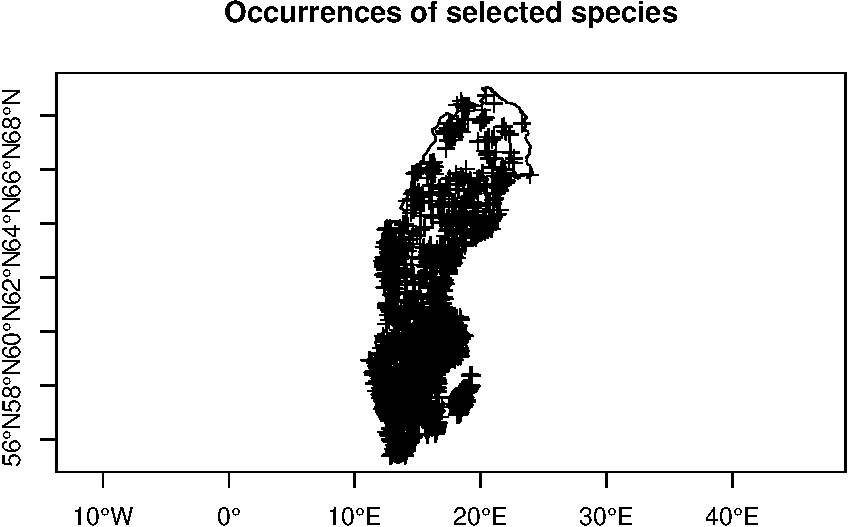
\includegraphics{tutorial_1_files/figure-latex/unnamed-chunk-8-1.pdf}

As you see in our plot we didn't plot a map, but instead a simple
coordinate system. However the spatial relationships between the points
are plotted in the correct ratios based on their latitude and longitude
coordinates. In principle, plotting points on a map is just plotting in
a regular coordinate system (as above) with a fancy background.

\hypertarget{lines}{%
\paragraph{Lines}\label{lines}}

We can also plot \textbf{lines} connecting our dots from above, using
the \texttt{lines()} function. Here we are only \textbf{plotting} our
points as lines but later we will see how to define line objects, which
besides the point coordinate information also carry the information in
which order the points are connected. This can be used e.g.~to visualize
a time chronology of sampling.

\begin{Shaded}
\begin{Highlighting}[]
\CommentTok{# first plot the points just as we did previously}
\KeywordTok{plot}\NormalTok{(sampling_sites, }\DataTypeTok{cex=}\DecValTok{2}\NormalTok{, }\DataTypeTok{pch=}\DecValTok{20}\NormalTok{, }\DataTypeTok{col=}\StringTok{'red'}\NormalTok{, }\DataTypeTok{main=}\StringTok{'Sampling sites'}\NormalTok{)}
\CommentTok{# draw lines between data points}
\KeywordTok{lines}\NormalTok{(sampling_sites, }\DataTypeTok{lwd=}\DecValTok{3}\NormalTok{, }\DataTypeTok{col=}\StringTok{'red'}\NormalTok{)}
\KeywordTok{text}\NormalTok{(sampling_sites, name, }\DataTypeTok{pos=}\DecValTok{4}\NormalTok{)}
\end{Highlighting}
\end{Shaded}

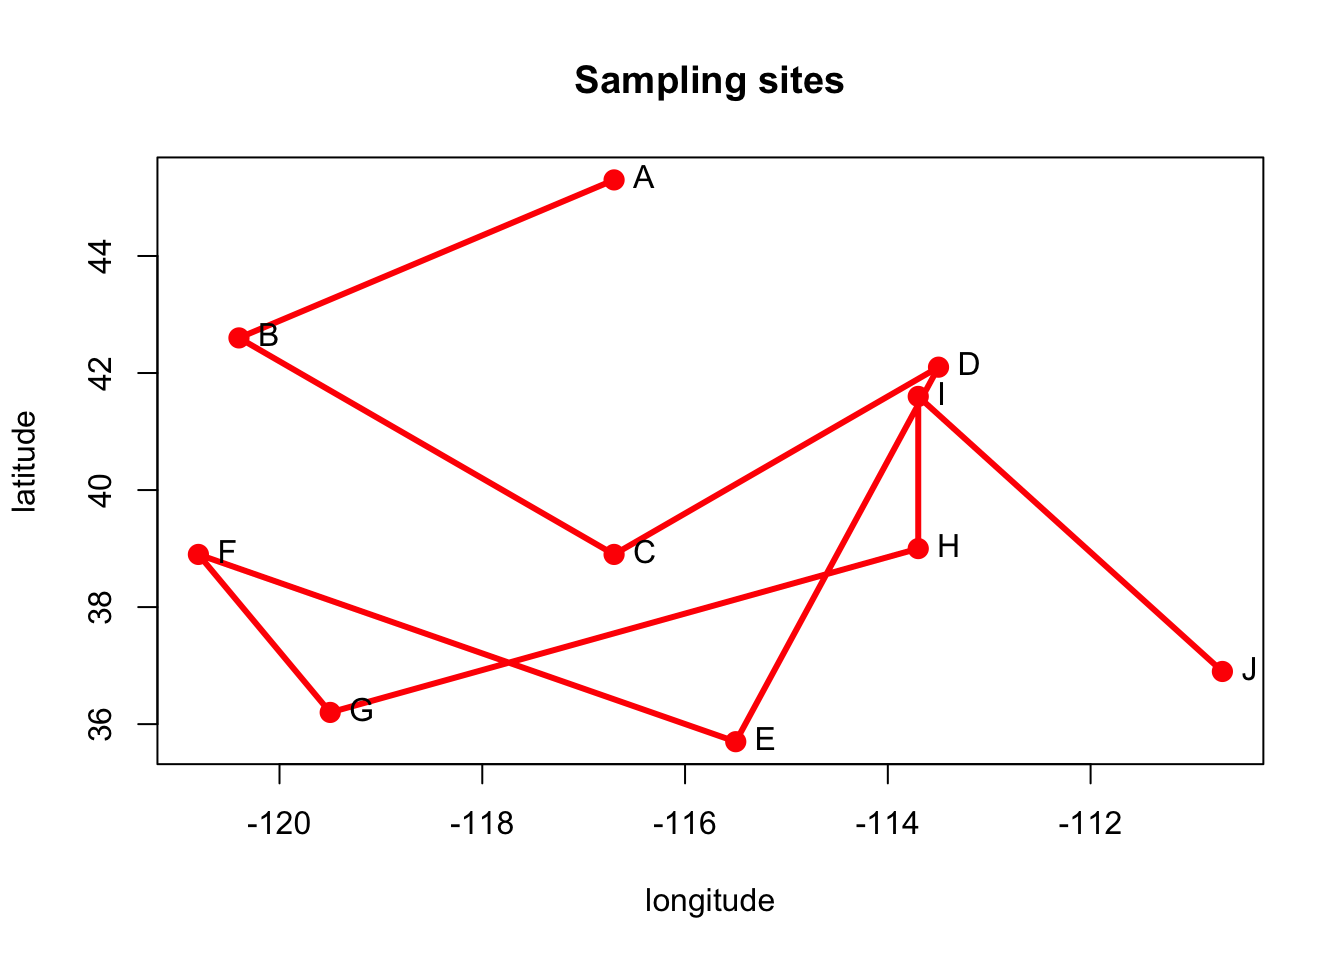
\includegraphics{tutorial_1_files/figure-latex/unnamed-chunk-9-1.pdf}

\hypertarget{polygons}{%
\paragraph{Polygons}\label{polygons}}

We can also plot a \textbf{polygon} from the same data, using the
\texttt{polygon()} function.

\begin{Shaded}
\begin{Highlighting}[]
\KeywordTok{plot}\NormalTok{(sampling_sites, }\DataTypeTok{cex=}\DecValTok{2}\NormalTok{, }\DataTypeTok{pch=}\DecValTok{20}\NormalTok{, }\DataTypeTok{col=}\StringTok{'red'}\NormalTok{, }\DataTypeTok{main=}\StringTok{'Sampling sites'}\NormalTok{)}
\KeywordTok{polygon}\NormalTok{(sampling_sites, }\DataTypeTok{col=}\StringTok{'blue'}\NormalTok{, }\DataTypeTok{border=}\StringTok{'light blue'}\NormalTok{)}
\KeywordTok{text}\NormalTok{(sampling_sites, name, }\DataTypeTok{pos=}\DecValTok{4}\NormalTok{)}
\end{Highlighting}
\end{Shaded}

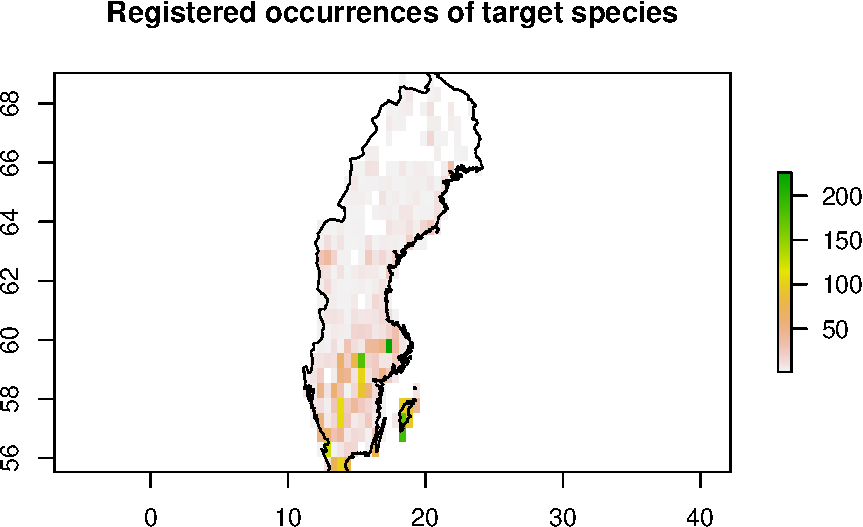
\includegraphics{tutorial_1_files/figure-latex/unnamed-chunk-10-1.pdf}

As you can see, also in case of polygons it matters in which order the
points are stored. Let's reorder our data points and see how the polygon
changes. For reordering an array we can just select the elements in the
desired order by using their indices. For example for an array
containing the 3 values `a',`b',and `c' named \texttt{my\_tiny\_array}
you can reorder the array having the 2nd element followed by the 3rd and
then the 1st like this:

\begin{Shaded}
\begin{Highlighting}[]
\NormalTok{my_tiny_array =}\StringTok{ }\KeywordTok{c}\NormalTok{(}\StringTok{'a'}\NormalTok{,}\StringTok{'b'}\NormalTok{,}\StringTok{'c'}\NormalTok{)}
\NormalTok{my_tiny_array[}\KeywordTok{c}\NormalTok{(}\DecValTok{2}\NormalTok{,}\DecValTok{3}\NormalTok{,}\DecValTok{1}\NormalTok{)]}
\end{Highlighting}
\end{Shaded}

\begin{verbatim}
## [1] "b" "c" "a"
\end{verbatim}

Now we want to do the same for our coordinate array
\texttt{sampling\_sites}. Since this is a 2D array we need to specify
rows and columns when selecting indices. Since we want to extract both
columns and only reorder the lines in our \texttt{sampling\_sites}
array, we specify the new order of row indices followed by a comma.

\begin{Shaded}
\begin{Highlighting}[]
\NormalTok{reordered_sampling_sites =}\StringTok{ }\NormalTok{sampling_sites[ }\KeywordTok{c}\NormalTok{(}\DecValTok{1}\NormalTok{,}\DecValTok{2}\NormalTok{,}\DecValTok{6}\NormalTok{,}\DecValTok{7}\NormalTok{,}\DecValTok{5}\NormalTok{,}\DecValTok{10}\NormalTok{,}\DecValTok{8}\NormalTok{,}\DecValTok{3}\NormalTok{,}\DecValTok{9}\NormalTok{,}\DecValTok{4}\NormalTok{), ]}
\KeywordTok{plot}\NormalTok{(reordered_sampling_sites, }\DataTypeTok{cex=}\DecValTok{2}\NormalTok{, }\DataTypeTok{pch=}\DecValTok{20}\NormalTok{, }\DataTypeTok{col=}\StringTok{'red'}\NormalTok{, }\DataTypeTok{main=}\StringTok{'Sampling sites'}\NormalTok{)}
\KeywordTok{polygon}\NormalTok{(reordered_sampling_sites, }\DataTypeTok{col=}\StringTok{'blue'}\NormalTok{, }\DataTypeTok{border=}\StringTok{'light blue'}\NormalTok{)}
\KeywordTok{text}\NormalTok{(sampling_sites, name, }\DataTypeTok{pos=}\DecValTok{4}\NormalTok{)}
\end{Highlighting}
\end{Shaded}

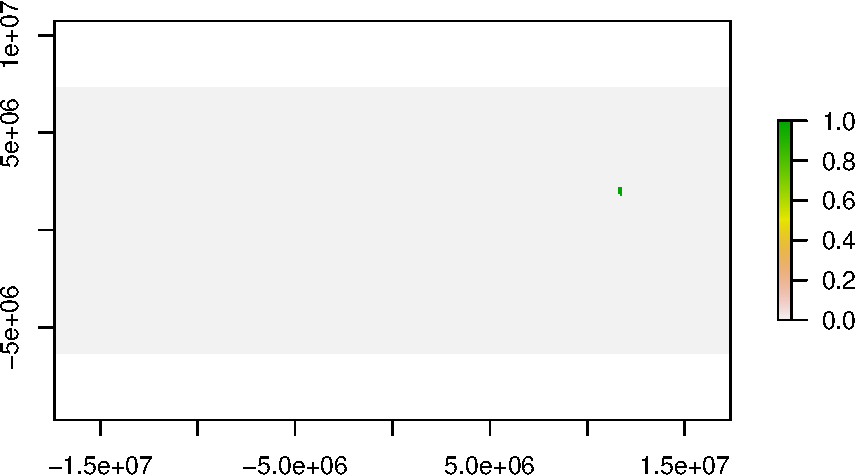
\includegraphics{tutorial_1_files/figure-latex/unnamed-chunk-12-1.pdf}

\hypertarget{defining-spatial-objects}{%
\paragraph{Defining spatial objects}\label{defining-spatial-objects}}

So far we have only worked with simple data points stored in arrays.
However, different data object types exist that are specifically
designed to handle spatial data. Some of the most commonly used objects
are defined in the \texttt{sp} package. For vector data, the basic types
are the \texttt{SpatialPoints()}, \texttt{SpatialLines()}, and
\texttt{SpatialPolygons()}. These data objects only represent
geometries. To also store attributes, additional data objects are
available with these names plus `DataFrame', for example,
\texttt{SpatialPolygonsDataFrame()} and
\texttt{SpatialPointsDataFrame()}. The advantage of this over e.g.~just
storing your coordinates in array form as we did so far, is that these
data spatial objects have several useful functions, for example you can
define the coordinate reference system of your coordinates in the
spatial object, which makes it easy to later on transform your
coordinates into another coordinate projection (you will see examples of
that later on). Also most spatial functions you may be using to process
or plot your data may require your data to be stored as spatial objects.
Let's store our coordinates as a \texttt{SpatialPoints()} object and
inspect the content and structure of this object with the
\texttt{showDefault()} function.

\begin{Shaded}
\begin{Highlighting}[]
\KeywordTok{library}\NormalTok{(sp)}
\NormalTok{pts <-}\StringTok{ }\KeywordTok{SpatialPoints}\NormalTok{(sampling_sites)}
\CommentTok{# use the showDefault() function to view th content of the object (works for any type of object in R)}
\KeywordTok{showDefault}\NormalTok{(pts)}
\end{Highlighting}
\end{Shaded}

\begin{verbatim}
## An object of class "SpatialPoints"
## Slot "coords":
##       longitude latitude
##  [1,]    -116.7     45.3
##  [2,]    -120.4     42.6
##  [3,]    -116.7     38.9
##  [4,]    -113.5     42.1
##  [5,]    -115.5     35.7
##  [6,]    -120.8     38.9
##  [7,]    -119.5     36.2
##  [8,]    -113.7     39.0
##  [9,]    -113.7     41.6
## [10,]    -110.7     36.9
## 
## Slot "bbox":
##              min    max
## longitude -120.8 -110.7
## latitude    35.7   45.3
## 
## Slot "proj4string":
## CRS arguments: NA
\end{verbatim}

You see that besides the coordinate pairs we defined, this object
contains information about the bounding box \texttt{bbox}, which defines
the smallest rectangle containing all of your points. It also contains
the currently empty slot \texttt{proj4string}, which is where you can
store the coordinate reference system of your points, which we will do
in a little bit. You will also notice when plotting the points that the
plot will look a bit different than before (e.g.~it's lacking the x and
y axis). The reason for that is that the default plotting options for
\texttt{SpatialPoints()} objects are different than those of simple
numeric arrays (which makes sense because often when you want to plot
points on a map, you may not wany the x-axis and y-axis to show).

\begin{Shaded}
\begin{Highlighting}[]
\KeywordTok{plot}\NormalTok{(pts, }\DataTypeTok{cex=}\DecValTok{2}\NormalTok{, }\DataTypeTok{pch=}\DecValTok{20}\NormalTok{, }\DataTypeTok{col=}\StringTok{'red'}\NormalTok{, }\DataTypeTok{main=}\StringTok{'Sampling sites'}\NormalTok{)}
\end{Highlighting}
\end{Shaded}

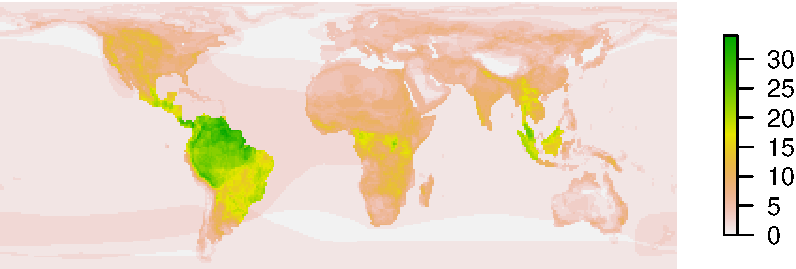
\includegraphics{tutorial_1_files/figure-latex/unnamed-chunk-14-1.pdf}

You can extract the additional values stored in the
\texttt{SpatialPoints()} object, e.g.~the coordinates of the bounding
box, like this:

\begin{Shaded}
\begin{Highlighting}[]
\NormalTok{box =}\StringTok{ }\KeywordTok{bbox}\NormalTok{(pts)}
\NormalTok{box}
\end{Highlighting}
\end{Shaded}

\begin{verbatim}
##              min    max
## longitude -120.8 -110.7
## latitude    35.7   45.3
\end{verbatim}

Let's plot the bounding box with our coordinates to see what it looks
like. You can use the \texttt{rect()} function to plot a simple
rectangle given the x and y coordinates of two opposing corner points:

\begin{Shaded}
\begin{Highlighting}[]
\KeywordTok{plot}\NormalTok{(pts, }\DataTypeTok{cex=}\DecValTok{2}\NormalTok{, }\DataTypeTok{pch=}\DecValTok{20}\NormalTok{, }\DataTypeTok{col=}\StringTok{'red'}\NormalTok{, }\DataTypeTok{main=}\StringTok{'Sampling sites'}\NormalTok{)}
\KeywordTok{rect}\NormalTok{(box[}\DecValTok{1}\NormalTok{],box[}\DecValTok{2}\NormalTok{],box[}\DecValTok{3}\NormalTok{],box[}\DecValTok{4}\NormalTok{])}
\end{Highlighting}
\end{Shaded}

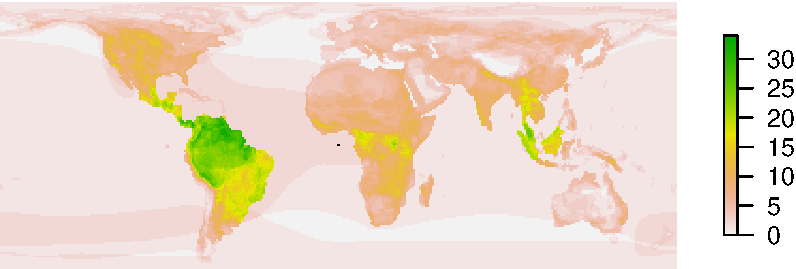
\includegraphics{tutorial_1_files/figure-latex/unnamed-chunk-16-1.pdf}

Let's now use the \texttt{SpatialPointsDataFrame()} function to define a
spatial object containing additional information about the samples
(sample name and measured body size). For this we first store the data
in a dataframe and then assign it to the
\texttt{SpatialPointsDataFrame()} object together with the coordinates:

\begin{Shaded}
\begin{Highlighting}[]
\NormalTok{additional_data <-}\StringTok{ }\KeywordTok{data.frame}\NormalTok{(}\DataTypeTok{sample_name=}\NormalTok{name, }\DataTypeTok{body_size=}\NormalTok{body_size)}
\NormalTok{ptsdf <-}\StringTok{ }\KeywordTok{SpatialPointsDataFrame}\NormalTok{(pts, }\DataTypeTok{data=}\NormalTok{additional_data)}
\KeywordTok{showDefault}\NormalTok{(ptsdf)}
\end{Highlighting}
\end{Shaded}

\begin{verbatim}
## An object of class "SpatialPointsDataFrame"
## Slot "data":
##    sample_name body_size
## 1            A        11
## 2            B        15
## 3            C        17
## 4            D        19
## 5            E        22
## 6            F        12
## 7            G        21
## 8            H        14
## 9            I         9
## 10           J        18
## 
## Slot "coords.nrs":
## numeric(0)
## 
## Slot "coords":
##       longitude latitude
##  [1,]    -116.7     45.3
##  [2,]    -120.4     42.6
##  [3,]    -116.7     38.9
##  [4,]    -113.5     42.1
##  [5,]    -115.5     35.7
##  [6,]    -120.8     38.9
##  [7,]    -119.5     36.2
##  [8,]    -113.7     39.0
##  [9,]    -113.7     41.6
## [10,]    -110.7     36.9
## 
## Slot "bbox":
##              min    max
## longitude -120.8 -110.7
## latitude    35.7   45.3
## 
## Slot "proj4string":
## CRS arguments: NA
\end{verbatim}

Now we'll use a different function to create a spatial line object using
the \texttt{spLines()} function. For this we first need to load the
package \texttt{raster}. We'll also make up some new data, in order to
have different data points than for the \texttt{SpatialPoints} object
from above:

\begin{Shaded}
\begin{Highlighting}[]
\KeywordTok{library}\NormalTok{(raster)}
\CommentTok{# make up new data}
\NormalTok{lon <-}\StringTok{ }\KeywordTok{c}\NormalTok{(}\OperatorTok{-}\FloatTok{116.8}\NormalTok{, }\FloatTok{-114.2}\NormalTok{, }\FloatTok{-112.9}\NormalTok{, }\FloatTok{-111.9}\NormalTok{, }\FloatTok{-114.2}\NormalTok{, }\FloatTok{-115.4}\NormalTok{, }\FloatTok{-117.7}\NormalTok{)}
\NormalTok{lat <-}\StringTok{ }\KeywordTok{c}\NormalTok{(}\FloatTok{41.3}\NormalTok{, }\FloatTok{42.9}\NormalTok{, }\FloatTok{42.4}\NormalTok{, }\FloatTok{39.8}\NormalTok{, }\FloatTok{37.6}\NormalTok{, }\FloatTok{38.3}\NormalTok{, }\FloatTok{37.6}\NormalTok{)}
\NormalTok{lonlat <-}\StringTok{ }\KeywordTok{cbind}\NormalTok{(lon, lat)}
\CommentTok{# store data as spatial lines object}
\NormalTok{lns <-}\StringTok{ }\KeywordTok{spLines}\NormalTok{(lonlat)}
\NormalTok{lns}
\end{Highlighting}
\end{Shaded}

\begin{verbatim}
## class       : SpatialLines 
## features    : 1 
## extent      : -117.7, -111.9, 37.6, 42.9  (xmin, xmax, ymin, ymax)
## coord. ref. : NA
\end{verbatim}

Now if you plot this \texttt{spLines()} object, the plot function will
automatically know to plot it as lines and not as points:

\begin{Shaded}
\begin{Highlighting}[]
\KeywordTok{plot}\NormalTok{(lns)}
\end{Highlighting}
\end{Shaded}

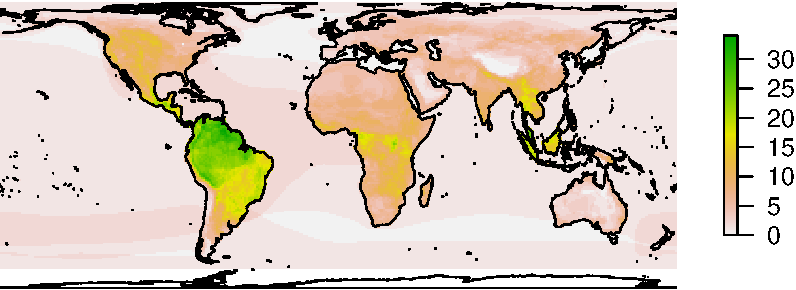
\includegraphics{tutorial_1_files/figure-latex/unnamed-chunk-19-1.pdf}

Similarly to the lines object, we can use the same points to create a
polygon using the \texttt{spPolygons()} function:

\begin{Shaded}
\begin{Highlighting}[]
\NormalTok{pols <-}\StringTok{ }\KeywordTok{spPolygons}\NormalTok{(lonlat)}
\NormalTok{pols}
\end{Highlighting}
\end{Shaded}

\begin{verbatim}
## class       : SpatialPolygons 
## features    : 1 
## extent      : -117.7, -111.9, 37.6, 42.9  (xmin, xmax, ymin, ymax)
## coord. ref. : NA
\end{verbatim}

Now let's plot the polygon and on top of it the spatial points form
earlier.

\begin{Shaded}
\begin{Highlighting}[]
\CommentTok{#plot(pols, axes=TRUE, las=1)}
\KeywordTok{plot}\NormalTok{(pts, }\DataTypeTok{col=}\StringTok{'black'}\NormalTok{, }\DataTypeTok{pch=}\DecValTok{20}\NormalTok{, }\DataTypeTok{cex=}\DecValTok{2}\NormalTok{,}\DataTypeTok{axes=}\OtherTok{TRUE}\NormalTok{)}
\KeywordTok{plot}\NormalTok{(pols, }\DataTypeTok{border=}\StringTok{'brown'}\NormalTok{, }\DataTypeTok{col=}\StringTok{'lightgreen'}\NormalTok{, }\DataTypeTok{lwd=}\DecValTok{3}\NormalTok{,}\DataTypeTok{add=}\NormalTok{T)}
\KeywordTok{plot}\NormalTok{(pts, }\DataTypeTok{col=}\StringTok{'black'}\NormalTok{, }\DataTypeTok{pch=}\DecValTok{20}\NormalTok{, }\DataTypeTok{cex=}\DecValTok{2}\NormalTok{,}\DataTypeTok{add=}\NormalTok{T)}
\end{Highlighting}
\end{Shaded}

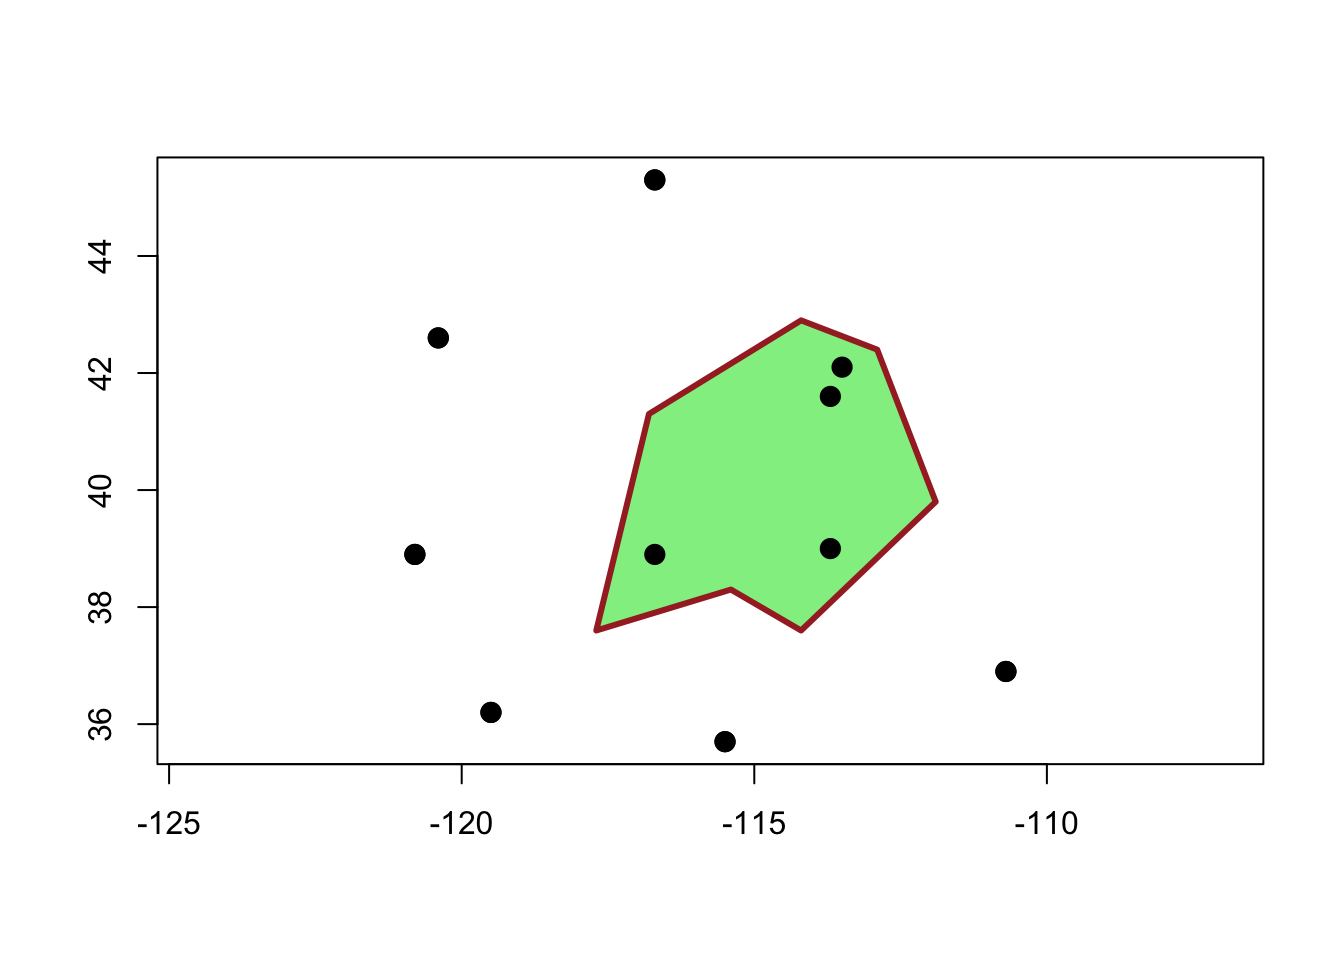
\includegraphics{tutorial_1_files/figure-latex/unnamed-chunk-21-1.pdf}

You may have noticed that this time we don't have to use the specific
plotting functions \texttt{polygon()} or \texttt{lines()} to tell R what
kind of object we want to plot, but instead we are simply using the
\texttt{plot()} function and R plots the data in the correct form by
default, since this information is contained in the specific types of
spatial objects we defined.

\hypertarget{rasters}{%
\subsubsection{2. Rasters}\label{rasters}}

Now let'swork a bit with rasters. The first type of raster object we
will work with is called \texttt{RasterLayer()} and is defined in the
\texttt{raster} library.

A RasterLayer object represents single-layer raster data. A RasterLayer
object always stores a number of fundamental parameters that describe
it. These include the number of columns and rows, the spatial extent,
and the Coordinate Reference System.

Here we create a RasterLayer from scratch. But note that in most cases
where real data is analyzed, these objects are read from a file. We
define a raster with 10 rows and 10 columns and we define the extent of
the raster on the x-axis (longitude) and on the y-axis (latitude).

\begin{Shaded}
\begin{Highlighting}[]
\KeywordTok{library}\NormalTok{(raster)}
\NormalTok{rast <-}\StringTok{ }\KeywordTok{raster}\NormalTok{(}\DataTypeTok{ncol=}\DecValTok{10}\NormalTok{, }\DataTypeTok{nrow=}\DecValTok{10}\NormalTok{, }\DataTypeTok{xmn=}\OperatorTok{-}\DecValTok{150}\NormalTok{, }\DataTypeTok{xmx=}\OperatorTok{-}\DecValTok{80}\NormalTok{, }\DataTypeTok{ymn=}\DecValTok{20}\NormalTok{, }\DataTypeTok{ymx=}\DecValTok{60}\NormalTok{)}
\NormalTok{rast}
\end{Highlighting}
\end{Shaded}

\begin{verbatim}
## class       : RasterLayer 
## dimensions  : 10, 10, 100  (nrow, ncol, ncell)
## resolution  : 7, 4  (x, y)
## extent      : -150, -80, 20, 60  (xmin, xmax, ymin, ymax)
## coord. ref. : +proj=longlat +datum=WGS84 +ellps=WGS84 +towgs84=0,0,0
\end{verbatim}

You can see in the last line of the output that by default the
\texttt{raster()} function created the raster using the coordinate
reference system \texttt{+proj=longlat\ +datum=WGS84}. We will learn
later what that means.

So far the object we created represents only a skeleton of a raster data
set. That means, we have defined information about its location,
resolution, etc., but there are no values associated with it. Let's fill
the skeleton with some made up data. In this case we assign a vector of
random numbers (generated from a uniform distribution using the
\texttt{runif()} function) with a length that is equal to the number of
cells of the RasterLayer.

\textbf{Exploring the raster object:} Just as we did earlier, we can use
the \texttt{showDefault()} function again to explore the contents of the
raster object. Executing \texttt{showDefault(rast)} will show you all
the available information stored in the raster object that we just
defined. Any of the `Slots' that are listed as output of that function
are values that can be accessed by calling the name of the slot followed
by the name of the raster object in parantheses. For example you will
find the slot \texttt{nrows} in the output of the
\texttt{showDefault(rast)} command and you can extract that information
specifically with \texttt{ncol(rast)}.

You can determine the number of cells in your raster using
\texttt{ncell()}:

\begin{Shaded}
\begin{Highlighting}[]
\KeywordTok{ncell}\NormalTok{(rast)}
\end{Highlighting}
\end{Shaded}

\begin{verbatim}
## [1] 100
\end{verbatim}

Now let's create as many random numbers (between 0 and 1) as we have
cells in our raster:

\begin{Shaded}
\begin{Highlighting}[]
\NormalTok{raster_values =}\StringTok{ }\KeywordTok{runif}\NormalTok{(}\KeywordTok{ncell}\NormalTok{(rast))}
\NormalTok{raster_values}
\end{Highlighting}
\end{Shaded}

\begin{verbatim}
##   [1] 0.884376075 0.903862083 0.671362405 0.599870021 0.835478926
##   [6] 0.926523584 0.095431591 0.992607101 0.665591696 0.891744261
##  [11] 0.592577511 0.903228687 0.471157019 0.668992862 0.308617167
##  [16] 0.939480910 0.323837533 0.344436643 0.435098477 0.247008779
##  [21] 0.043818521 0.207123006 0.380147703 0.830941045 0.043181320
##  [26] 0.182630000 0.176790955 0.192392648 0.983401231 0.137250434
##  [31] 0.409988229 0.541147036 0.277448714 0.942606119 0.125970988
##  [36] 0.325446599 0.720267082 0.441816681 0.551561612 0.553297165
##  [41] 0.179322024 0.889273187 0.405722704 0.781701899 0.822388253
##  [46] 0.447078546 0.016234494 0.482852856 0.280788946 0.228518850
##  [51] 0.591143204 0.472886364 0.129328642 0.986931604 0.735316761
##  [56] 0.369630401 0.873237981 0.131640598 0.165255970 0.107351613
##  [61] 0.090989992 0.627320934 0.671711824 0.746207850 0.810541146
##  [66] 0.525938306 0.063900785 0.505032246 0.139079239 0.937037354
##  [71] 0.022363529 0.352050834 0.652673538 0.813805774 0.795178396
##  [76] 0.556039578 0.424779854 0.351808239 0.322324013 0.138651041
##  [81] 0.348549388 0.153984955 0.814157366 0.111726771 0.184340235
##  [86] 0.528970266 0.194364149 0.614404445 0.194290301 0.412433660
##  [91] 0.418664518 0.951191249 0.392978767 0.820497818 0.335803176
##  [96] 0.600424566 0.723563475 0.618591768 0.522158913 0.008727924
\end{verbatim}

Now we assign these random values to the raster using the
\texttt{values()} function and plot the raster with these new values.

\begin{Shaded}
\begin{Highlighting}[]
\KeywordTok{values}\NormalTok{(rast) =}\StringTok{ }\NormalTok{raster_values}
\KeywordTok{plot}\NormalTok{(rast)}
\end{Highlighting}
\end{Shaded}

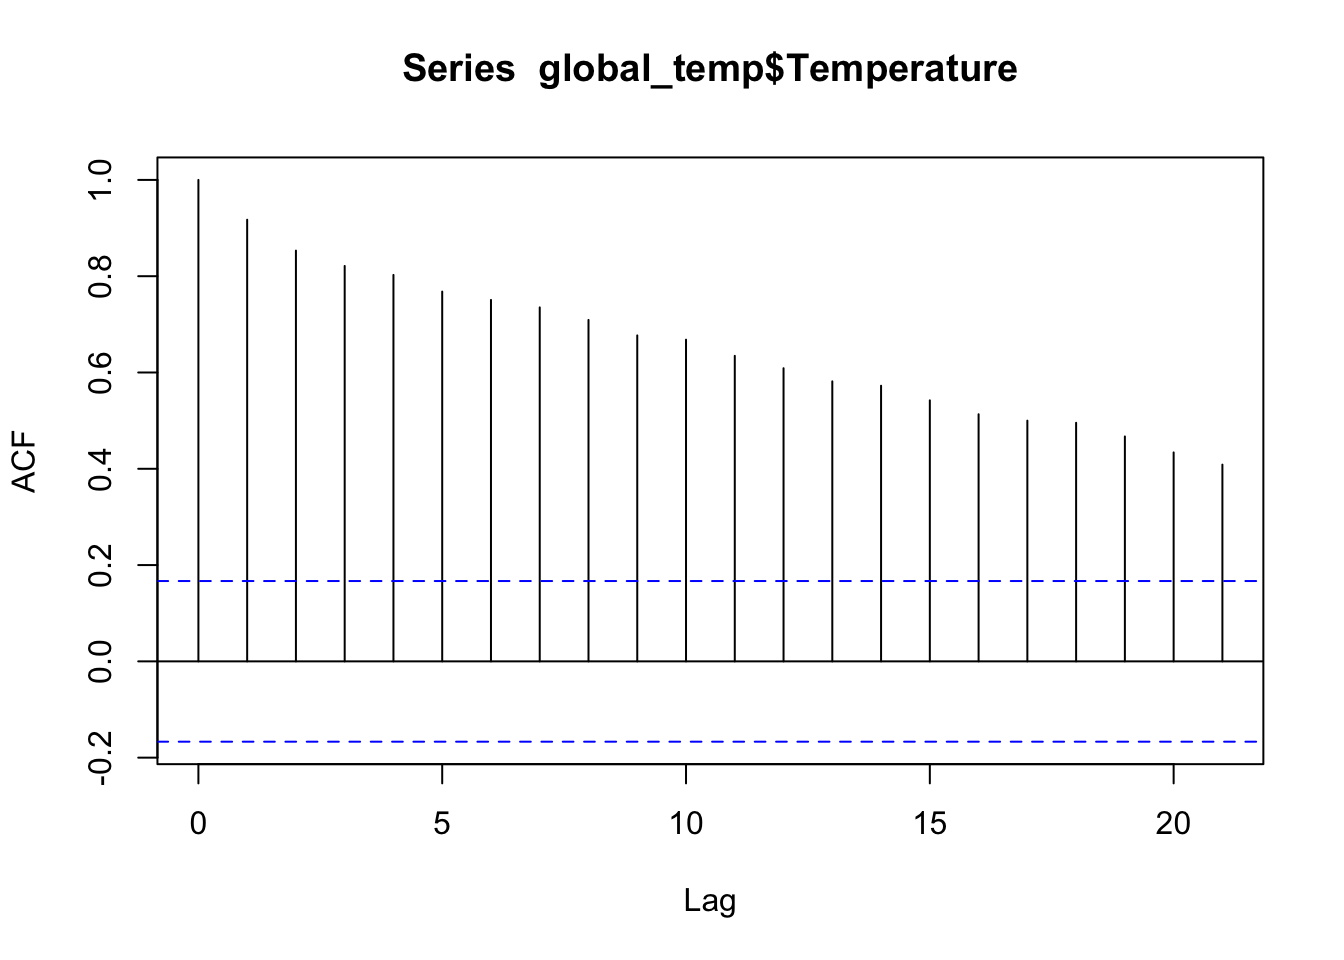
\includegraphics{tutorial_1_files/figure-latex/unnamed-chunk-25-1.pdf}

\textbf{Task:} Just because we can, and to demonstrate that the
coordinate systems of our created raster and our previously defined
spatial vector object match, let's plot the spatial polygon
\texttt{pols}and the spatial points \texttt{pts} on top of the raster.
Tip: you can use \texttt{add=T} in the plot command to add additional
layers on top of an existing plot without replacing the previous plot.
That way you can add multiple elements into the same plot. The final
plot should look like the one below.

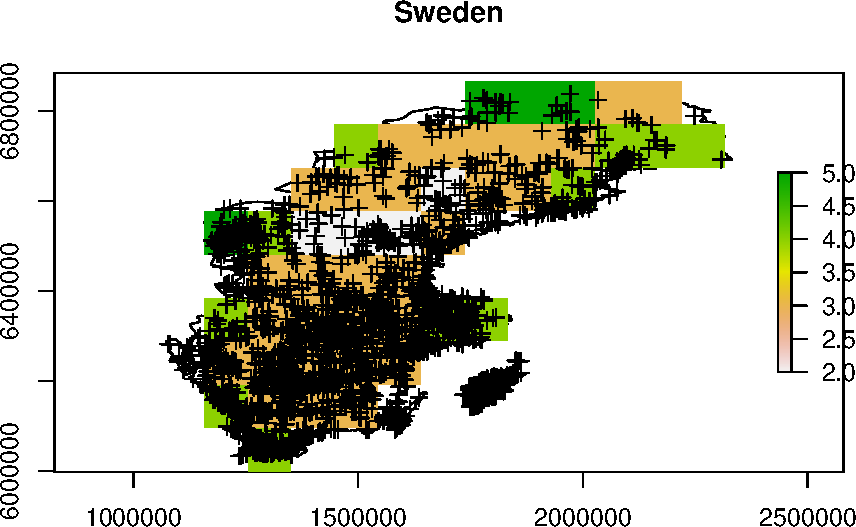
\includegraphics{tutorial_1_files/figure-latex/unnamed-chunk-26-1.pdf}

\hypertarget{reading-spatial-data-from-file}{%
\subsubsection{3. Reading spatial data from
file}\label{reading-spatial-data-from-file}}

We can use the \texttt{readShapePoly()} function in order to read a
shape file as a vectorized polygon into R. A shape file is usually made
up of at least four parts. The .SHP, the .DBF, the .PRJ and the .SHX.

\begin{itemize}
\tightlist
\item
  \textbf{SHP:} This file contains the geometry of each feature.
\item
  \textbf{DBF:} This is a database file which contains the attribute
  data for all of the features in the dataset. The database file is very
  similar to a sheet in a spreadsheet and can even be opened in Excel.
\item
  \textbf{SHX:} The .shx is the spatial index, it allows spatial
  programs to find features within the .SHP file more quickly.
\item
  \textbf{PRJ:} The .prj is the projection file. It contains information
  about the ``projection'' and ``coordinate system'' the data uses.
\end{itemize}

Below we are going to read a shape file of the country shape of Germany,
downloaded from \href{http://www.diva-gis.org/gdata}{DIVA-GIS}. You can
open the link and download your own shape file or work with the example
data, which you can find in the data folder of the
\href{https://github.com/tobiashofmann88/spatial_R_course}{GitHub repo
of this course}. I recommend you download the whole complete GitHub repo
by clicking on the green `Clone or download' button and then `Download
as ZIP'.

Once you have downloaded a shape file from DIVA-GIS or from the course
GitHub repo, you can read the file into R using the \texttt{st\_read()}
function. To use this function we need to load the \texttt{sf} package
with \texttt{library(sf)}. To load the file, make sure that you provide
the correct file path from your current working directory.

\textbf{Finding files in R}: Providing the right filepath to a file in R
can be a bit difficult at the beginning when you're not used to finding
files by navigating through the file path system. A good starting point
is usually to check the current working directory. You can see your
working directory with \texttt{getwd()}. From here you need to provide
the path to where your file is stored. One nice feature about RStudio is
that is autocompletes paths once you start writing them. For using this
function just type `./' and then press the Tab button, which will show
you all available files and folders in your current directory. Choose
the folder you want to navigate to and press Tab again to show the
content of that folder. You can use \texttt{../} to navigate out of a
folder inot the parent directory. \textbf{Important note for Windows
users:} Instead of using \texttt{/} in the file path you will have to
use \texttt{\textbackslash{}\textbackslash{}}!

\begin{Shaded}
\begin{Highlighting}[]
\KeywordTok{library}\NormalTok{(sf)}
\NormalTok{germany =}\StringTok{ }\KeywordTok{st_read}\NormalTok{(}\StringTok{'../data/DEU_adm/DEU_adm0.shp'}\NormalTok{)}
\end{Highlighting}
\end{Shaded}

\begin{verbatim}
## Reading layer `DEU_adm0' from data source `/Users/tobias/GitHub/spatial_R_course/data/DEU_adm/DEU_adm0.shp' using driver `ESRI Shapefile'
## Simple feature collection with 1 feature and 70 fields
## geometry type:  MULTIPOLYGON
## dimension:      XY
## bbox:           xmin: 5.871619 ymin: 47.26986 xmax: 15.03811 ymax: 55.05653
## epsg (SRID):    4326
## proj4string:    +proj=longlat +datum=WGS84 +no_defs
\end{verbatim}

The object that is created by the \texttt{st\_read()} function is a
feature collection in \texttt{sf} format. You don;t need to bother fully
understanding this format for our purposes, but instead we will just
turn it into the now familiar \texttt{SpatialPolygons} format
(\texttt{SpatialPolygonsDataFrame} to be precise, which we'll look at a
bit closer below). You can do this by using the command
\texttt{as(my\_object,\ \textquotesingle{}Spatial\textquotesingle{})},
where \texttt{my\_object} in this case is our \texttt{sf} object called
\texttt{germany}:

\begin{Shaded}
\begin{Highlighting}[]
\NormalTok{germany_spatial =}\StringTok{ }\KeywordTok{as}\NormalTok{(germany, }\StringTok{'Spatial'}\NormalTok{)}
\NormalTok{germany_spatial}
\end{Highlighting}
\end{Shaded}

\begin{verbatim}
## class       : SpatialPolygonsDataFrame 
## features    : 1 
## extent      : 5.871619, 15.03811, 47.26986, 55.05653  (xmin, xmax, ymin, ymax)
## coord. ref. : +proj=longlat +datum=WGS84 +no_defs +ellps=WGS84 +towgs84=0,0,0 
## variables   : 70
## names       : ID_0, ISO,  NAME_0, OBJECTID_1, ISO3, NAME_ENGLI, NAME_ISO, NAME_FAO,  NAME_LOCAL, NAME_OBSOL, NAME_VARIA, NAME_NONLA, NAME_FRENC, NAME_SPANI, NAME_RUSSI, ... 
## value       :   86, DEU, Germany,         62,  DEU,    Germany,  GERMANY,  Germany, Deutschland,         NA,    Germany,         NA,  Allemagne,   Alemania,   Германия, ...
\end{verbatim}

\begin{Shaded}
\begin{Highlighting}[]
\NormalTok{(germany_spatial)}
\end{Highlighting}
\end{Shaded}

\begin{verbatim}
## class       : SpatialPolygonsDataFrame 
## features    : 1 
## extent      : 5.871619, 15.03811, 47.26986, 55.05653  (xmin, xmax, ymin, ymax)
## coord. ref. : +proj=longlat +datum=WGS84 +no_defs +ellps=WGS84 +towgs84=0,0,0 
## variables   : 70
## names       : ID_0, ISO,  NAME_0, OBJECTID_1, ISO3, NAME_ENGLI, NAME_ISO, NAME_FAO,  NAME_LOCAL, NAME_OBSOL, NAME_VARIA, NAME_NONLA, NAME_FRENC, NAME_SPANI, NAME_RUSSI, ... 
## value       :   86, DEU, Germany,         62,  DEU,    Germany,  GERMANY,  Germany, Deutschland,         NA,    Germany,         NA,  Allemagne,   Alemania,   Германия, ...
\end{verbatim}

Now let's plot the polygon object we just created:

\begin{Shaded}
\begin{Highlighting}[]
\KeywordTok{plot}\NormalTok{(germany_spatial,}\DataTypeTok{main=}\StringTok{'Germany'}\NormalTok{)}
\end{Highlighting}
\end{Shaded}

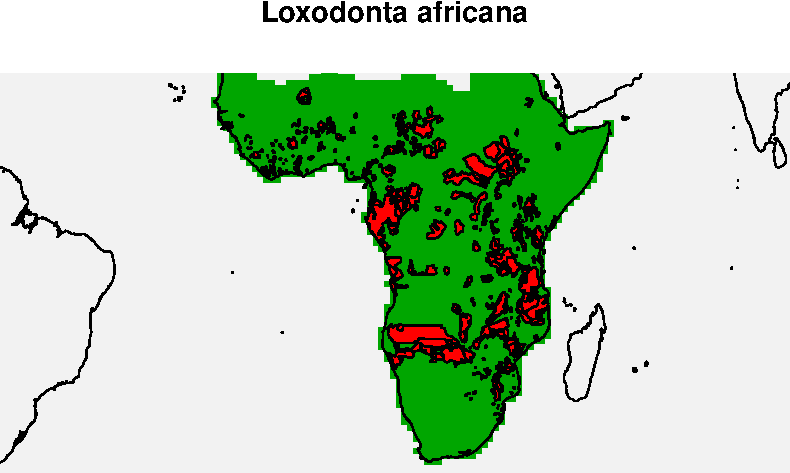
\includegraphics{tutorial_1_files/figure-latex/unnamed-chunk-29-1.pdf}

Similarly we can read raster data, using the \texttt{raster()} function.
In this example we are reading altitude information covering the area of
Germany, which we will use in combination with the shape file from
above:

\begin{Shaded}
\begin{Highlighting}[]
\NormalTok{germany_alt_raster =}\StringTok{ }\KeywordTok{raster}\NormalTok{(}\StringTok{'../data/DEU_alt/deu_alt.grd'}\NormalTok{)}
\KeywordTok{plot}\NormalTok{(germany_alt_raster,}\DataTypeTok{main=}\StringTok{'Altitude in meters above sea level'}\NormalTok{)}
\end{Highlighting}
\end{Shaded}

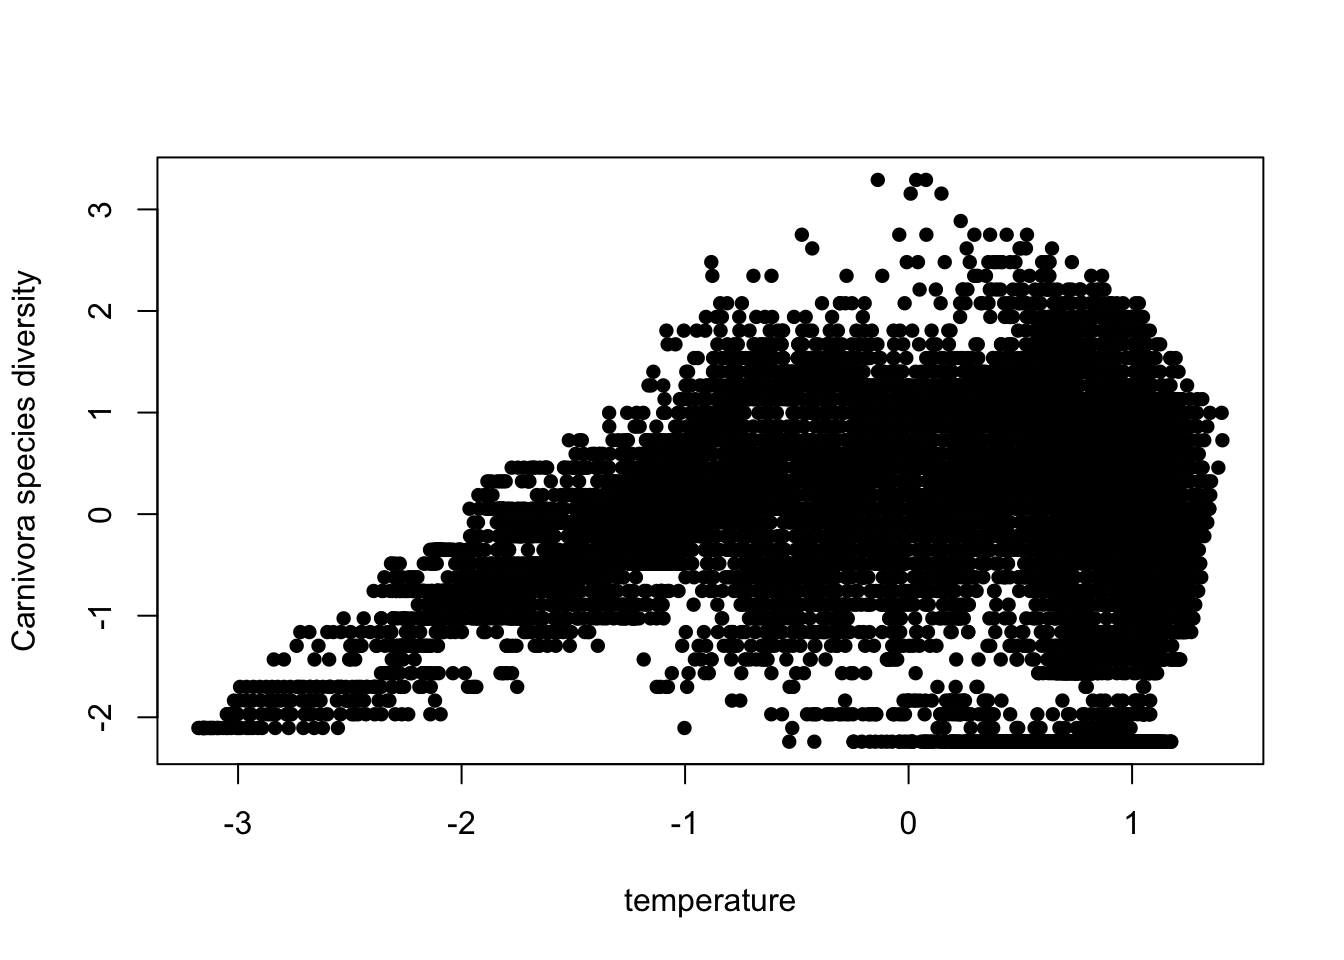
\includegraphics{tutorial_1_files/figure-latex/unnamed-chunk-30-1.pdf}

\textbf{Task:} The raster is a rectangular grid filled with values (just
as we did manually for the random value raster earlier in the tutorial).
Let's now plot the country borders of Germany (stored in the
\texttt{germany\_spatial} object) on top of the raster, just as you did
before when plotting our hand-made polygon on top of the random value
raster. Your plot should look like the one below.

\includegraphics{tutorial_1_files/figure-latex/unnamed-chunk-31-1.pdf}

\hypertarget{coordinate-reference-systems}{%
\subsubsection{4. Coordinate Reference
Systems}\label{coordinate-reference-systems}}

The reason why plotting the country borders of Germany on top of the
raster worked so smoothly is because both objects (the polygon and the
raster) are scaled in the same coordinate reference system (CRS). We
will work through an where the CRSs between two objects don't match, and
where they have to be adjusted first, in the next tutorial. For now, to
get a basic understanding what this is all about, please read the
sections 6.1 and 6.2 in
\href{http://rspatial.org/spatial/rst/6-crs.html}{this summary about
coordinate reference systems}, which explains the background about
different two-dimensional projections of geographic data.

\hypertarget{working-with-vector-data}{%
\subsubsection{5. Working with vector
data}\label{working-with-vector-data}}

Now we are going to play around with a map of Luxembourg in order to
demonstrate some of the basic polygon transformation and editing tools.

Let's first read the shape file and turn it into a spatial object, just
as we did before for the Germany shape file:

\begin{Shaded}
\begin{Highlighting}[]
\NormalTok{lux =}\StringTok{ }\KeywordTok{st_read}\NormalTok{(}\StringTok{'../data/luxembourg/lux.shp'}\NormalTok{)}
\end{Highlighting}
\end{Shaded}

\begin{verbatim}
## Reading layer `lux' from data source `/Users/tobias/GitHub/spatial_R_course/data/luxembourg/lux.shp' using driver `ESRI Shapefile'
## Simple feature collection with 12 features and 5 fields
## geometry type:  POLYGON
## dimension:      XY
## bbox:           xmin: 5.74414 ymin: 49.44781 xmax: 6.528252 ymax: 50.18162
## epsg (SRID):    4326
## proj4string:    +proj=longlat +datum=WGS84 +no_defs
\end{verbatim}

\begin{Shaded}
\begin{Highlighting}[]
\NormalTok{lux_spatial =}\StringTok{ }\KeywordTok{as}\NormalTok{(lux, }\StringTok{'Spatial'}\NormalTok{)}
\NormalTok{lux_spatial}
\end{Highlighting}
\end{Shaded}

\begin{verbatim}
## class       : SpatialPolygonsDataFrame 
## features    : 12 
## extent      : 5.74414, 6.528252, 49.44781, 50.18162  (xmin, xmax, ymin, ymax)
## coord. ref. : +proj=longlat +datum=WGS84 +no_defs +ellps=WGS84 +towgs84=0,0,0 
## variables   : 5
## names       : ID_1,     NAME_1, ID_2,   NAME_2, AREA 
## min values  :    1,   Diekirch,    1, Capellen,   76 
## max values  :    3, Luxembourg,   12,    Wiltz,  312
\end{verbatim}

The shape object is formatted as a \texttt{SpatialPolygonsDataFrame}.
Similarly to the \texttt{SpatialPointsDataFrame} from earlier in the
tutorial, a \texttt{SpatialPolygonsDataFrame} contains a list of
\texttt{SpatialPolygons}, as well as other data associated with these
polygons. This could for example be the polygons of different regions
within the country and the associated values could be things like name,
population, size, etc. of these individual regions. You can see from the
output of the above command (by just executing the name of the object:
\texttt{lux\_spatial}), that there are 12 features in this object. That
means that this \texttt{SpatialPolygonsDataFrame} contains 12 different
polygons, each based on it's own set of coordinates and associated with
it's own data. You can see the names of the different data columns that
are stored in the object using the \texttt{names()} function:

\begin{Shaded}
\begin{Highlighting}[]
\KeywordTok{names}\NormalTok{(lux_spatial)}
\end{Highlighting}
\end{Shaded}

\begin{verbatim}
## [1] "ID_1"   "NAME_1" "ID_2"   "NAME_2" "AREA"
\end{verbatim}

There are five different values associated with each polygon which are
stored in the columns
\texttt{ID\_1},\texttt{NAME\_1},\texttt{ID\_2},\texttt{NAME\_2},\texttt{AREA}.
When plotting the actual \texttt{sf} object \texttt{lux} (instead of the
\texttt{SpatialPolygonDataFrame} object \texttt{lux\_spatial}), the
default plotting function automatically puts out all layers and colors
the polygons by their values:

\begin{Shaded}
\begin{Highlighting}[]
\KeywordTok{plot}\NormalTok{(lux,}\DataTypeTok{axes =}\NormalTok{ T)}
\end{Highlighting}
\end{Shaded}

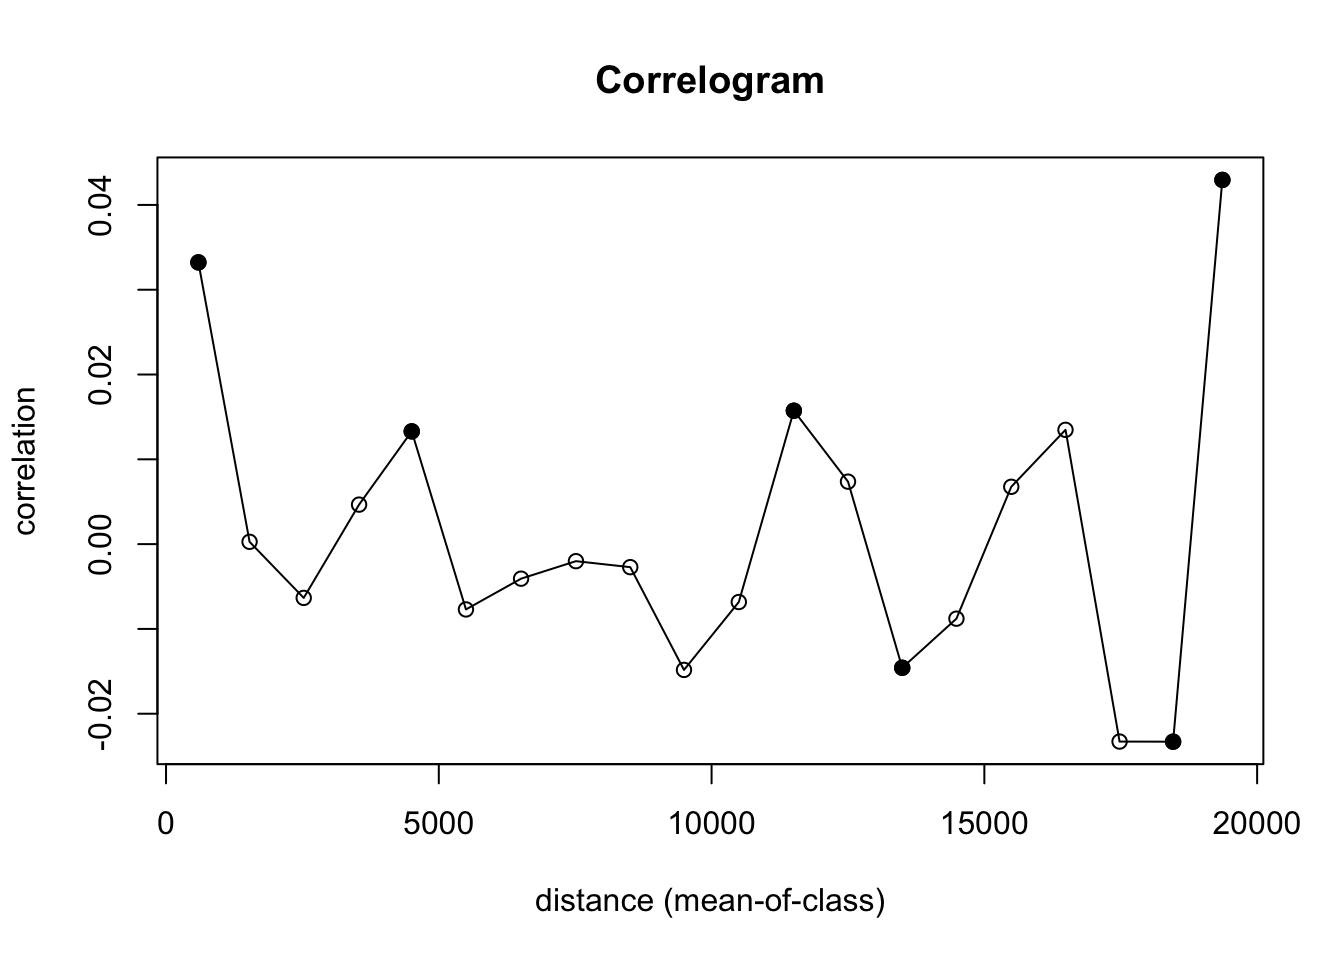
\includegraphics{tutorial_1_files/figure-latex/unnamed-chunk-34-1.pdf}

You can see that e.g. \texttt{NAME\_1} defines some larger regions, as
several neighbouring polygons share the same value for that data column,
while \texttt{NAME\_2} seems to define the names of the polygons we have
in our dataframe (more regional delimitations). We can select a single
layer by using the respective index in square brackets \texttt{{[}{]}}:

\begin{Shaded}
\begin{Highlighting}[]
\KeywordTok{plot}\NormalTok{(lux[}\DecValTok{4}\NormalTok{],}\DataTypeTok{axes =}\NormalTok{ T)}
\end{Highlighting}
\end{Shaded}

\includegraphics{tutorial_1_files/figure-latex/unnamed-chunk-35-1.pdf}

We can extract the values of a specific column like this:

\begin{Shaded}
\begin{Highlighting}[]
\NormalTok{lux}\OperatorTok{$}\NormalTok{NAME_}\DecValTok{2}
\end{Highlighting}
\end{Shaded}

\begin{verbatim}
##  [1] Clervaux         Diekirch         Redange          Vianden         
##  [5] Wiltz            Echternach       Remich           Grevenmacher    
##  [9] Capellen         Esch-sur-Alzette Luxembourg       Mersch          
## 12 Levels: Capellen Clervaux Diekirch Echternach ... Wiltz
\end{verbatim}

In some cases you may want to add a column of additional values to the
polygon object, e.g.~if you want to code which of these regions you have
sampled (\texttt{1} stands for sampled and \texttt{0} stands for not
sampled):

\begin{Shaded}
\begin{Highlighting}[]
\NormalTok{new_values =}\StringTok{ }\KeywordTok{c}\NormalTok{(}\DecValTok{0}\NormalTok{,}\DecValTok{1}\NormalTok{,}\DecValTok{1}\NormalTok{,}\DecValTok{0}\NormalTok{,}\DecValTok{1}\NormalTok{,}\DecValTok{0}\NormalTok{,}\DecValTok{1}\NormalTok{,}\DecValTok{1}\NormalTok{,}\DecValTok{0}\NormalTok{,}\DecValTok{0}\NormalTok{,}\DecValTok{0}\NormalTok{,}\DecValTok{1}\NormalTok{)}
\NormalTok{lux}\OperatorTok{$}\NormalTok{sampled_regions =}\StringTok{ }\NormalTok{new_values}
\KeywordTok{plot}\NormalTok{(lux[}\StringTok{'sampled_regions'}\NormalTok{],}\DataTypeTok{axes =}\NormalTok{ T)}
\end{Highlighting}
\end{Shaded}

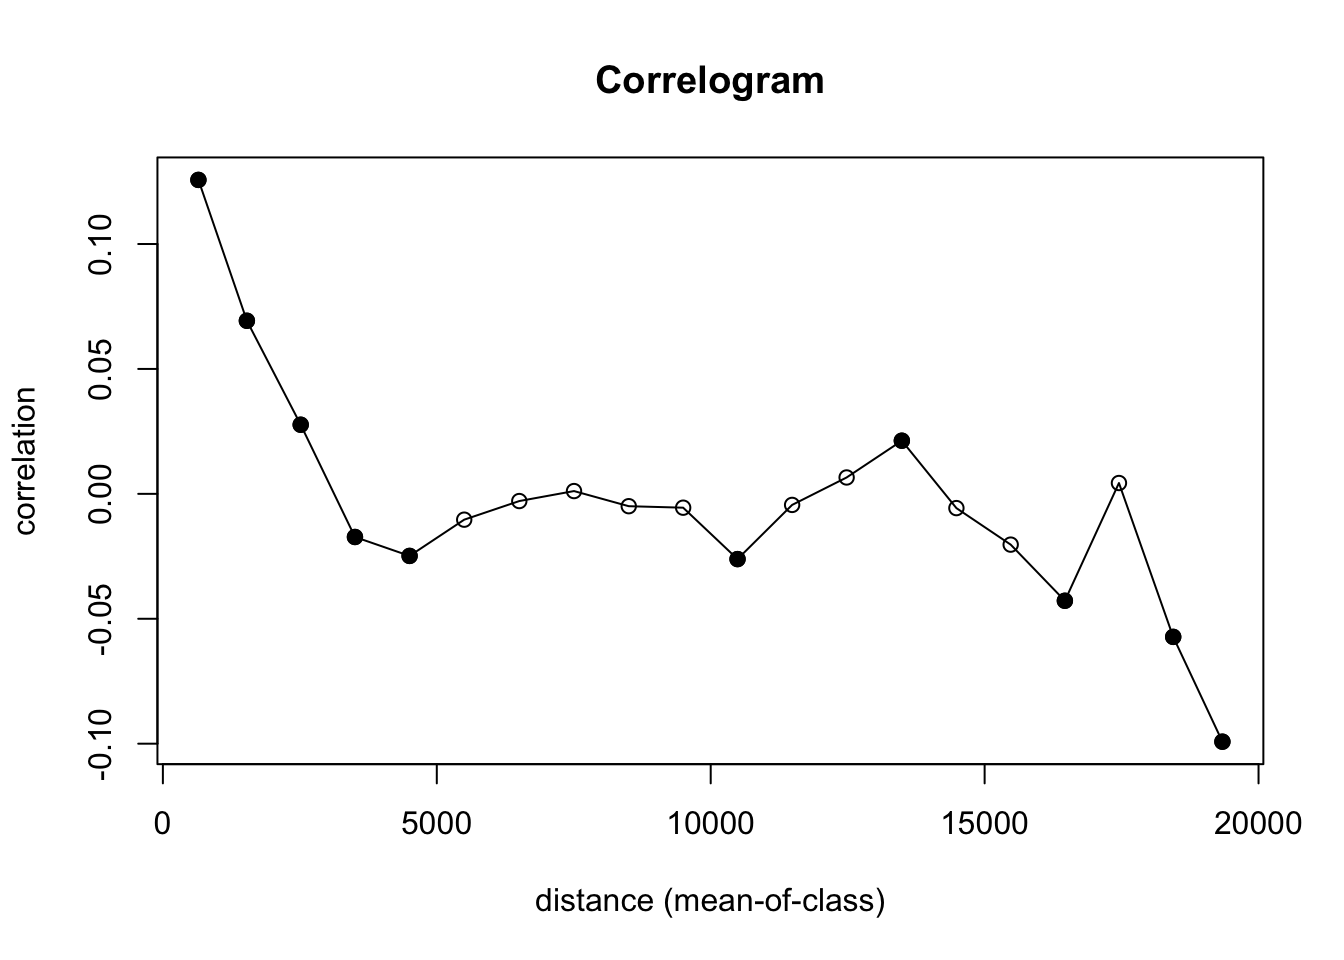
\includegraphics{tutorial_1_files/figure-latex/unnamed-chunk-37-1.pdf}

You can easily remove the column you just added above, using this
command

\begin{Shaded}
\begin{Highlighting}[]
\NormalTok{lux}\OperatorTok{$}\NormalTok{sampled_regions <-}\StringTok{ }\OtherTok{NULL}
\end{Highlighting}
\end{Shaded}

But for now let's add the new column again and selectively only plot
those areas that have not yet been sampled. We can do that by finding
the indexes \texttt{i} for the regions where our new column has the
value 0 (using the \texttt{which()} function and then extracting all of
those rows from the spatial data object:

\begin{Shaded}
\begin{Highlighting}[]
\NormalTok{new_values =}\StringTok{ }\KeywordTok{c}\NormalTok{(}\DecValTok{0}\NormalTok{,}\DecValTok{1}\NormalTok{,}\DecValTok{1}\NormalTok{,}\DecValTok{0}\NormalTok{,}\DecValTok{1}\NormalTok{,}\DecValTok{0}\NormalTok{,}\DecValTok{1}\NormalTok{,}\DecValTok{1}\NormalTok{,}\DecValTok{0}\NormalTok{,}\DecValTok{0}\NormalTok{,}\DecValTok{0}\NormalTok{,}\DecValTok{1}\NormalTok{)}
\NormalTok{lux}\OperatorTok{$}\NormalTok{sampled_regions =}\StringTok{ }\NormalTok{new_values}
\NormalTok{i <-}\StringTok{ }\KeywordTok{which}\NormalTok{(lux}\OperatorTok{$}\NormalTok{sampled_regions }\OperatorTok{==}\StringTok{ }\DecValTok{0}\NormalTok{)}
\NormalTok{g <-}\StringTok{ }\NormalTok{lux[i,]}
\KeywordTok{plot}\NormalTok{(g[}\StringTok{'sampled_regions'}\NormalTok{],}\DataTypeTok{main=}\StringTok{'Unsampled areas'}\NormalTok{,}\DataTypeTok{axes =}\NormalTok{ T)}
\end{Highlighting}
\end{Shaded}

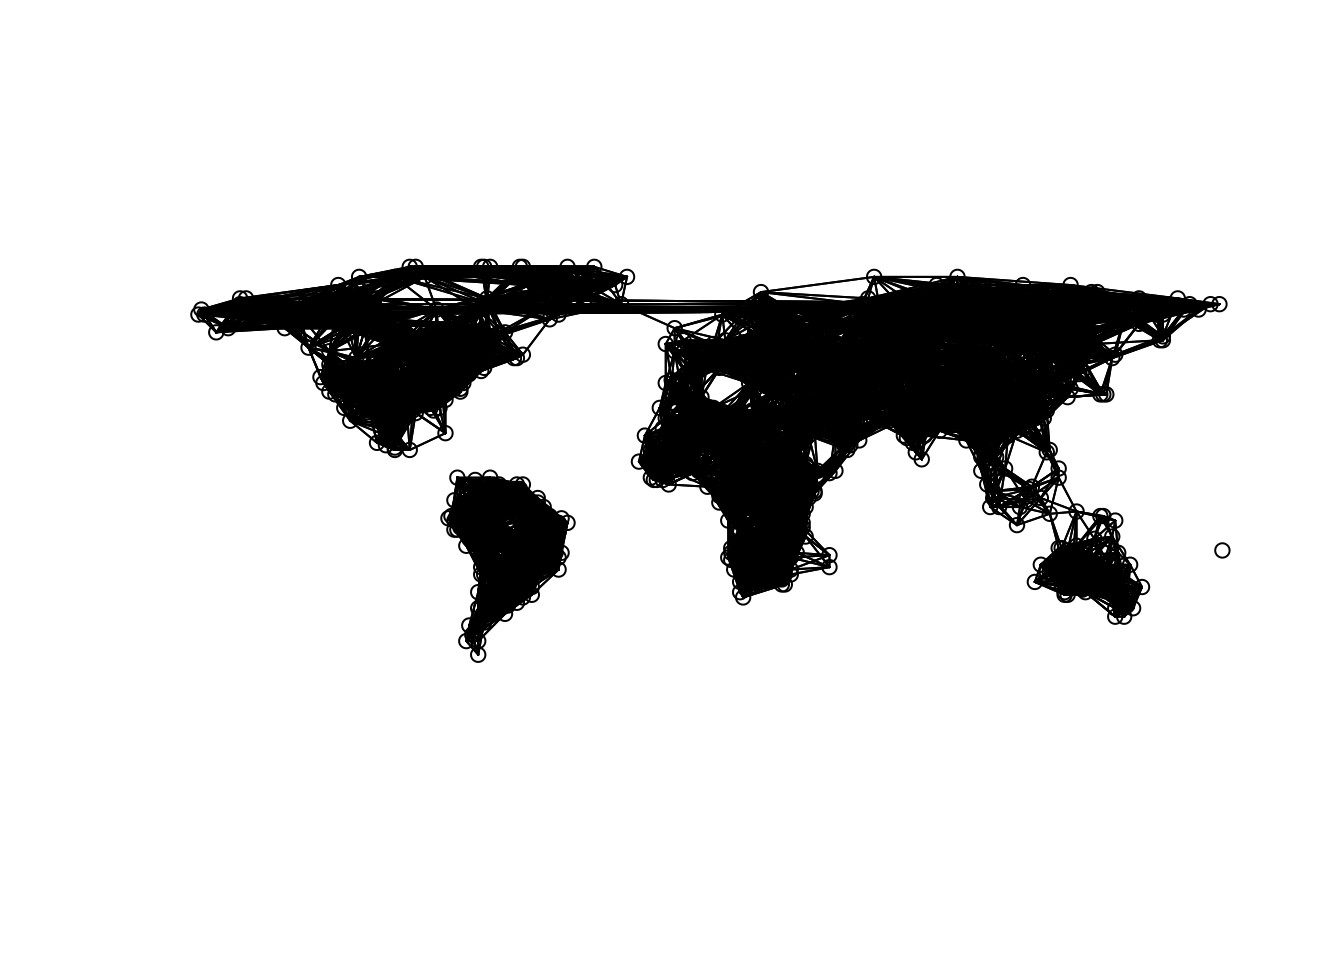
\includegraphics{tutorial_1_files/figure-latex/unnamed-chunk-39-1.pdf}

\hypertarget{creating-raster-over-polygon-and-convert-raster-back-to-polygon}{%
\subsubsection{Creating raster over polygon and convert raster back to
polygon}\label{creating-raster-over-polygon-and-convert-raster-back-to-polygon}}

Let's say we want to divide our Luxembourg polygon into 4 equally sized
cells. The easiest way to do this is to define a raster with 4 cells
that encompasses the whole polygon. You cna actually provide the raster
function with a spatial polygon and it will automatically create a
raster using the bounding box coordinates fo the polygon (note that we
are using the spatial object \texttt{lux\_spatial} again, not the sf
object \texttt{lux}):

\begin{Shaded}
\begin{Highlighting}[]
\NormalTok{z <-}\StringTok{ }\KeywordTok{raster}\NormalTok{(lux_spatial, }\DataTypeTok{nrow=}\DecValTok{2}\NormalTok{, }\DataTypeTok{ncol=}\DecValTok{2}\NormalTok{, }\DataTypeTok{vals=}\DecValTok{1}\OperatorTok{:}\DecValTok{4}\NormalTok{)}
\KeywordTok{plot}\NormalTok{(z)}
\KeywordTok{plot}\NormalTok{(lux_spatial,}\DataTypeTok{add=}\NormalTok{T)}
\end{Highlighting}
\end{Shaded}

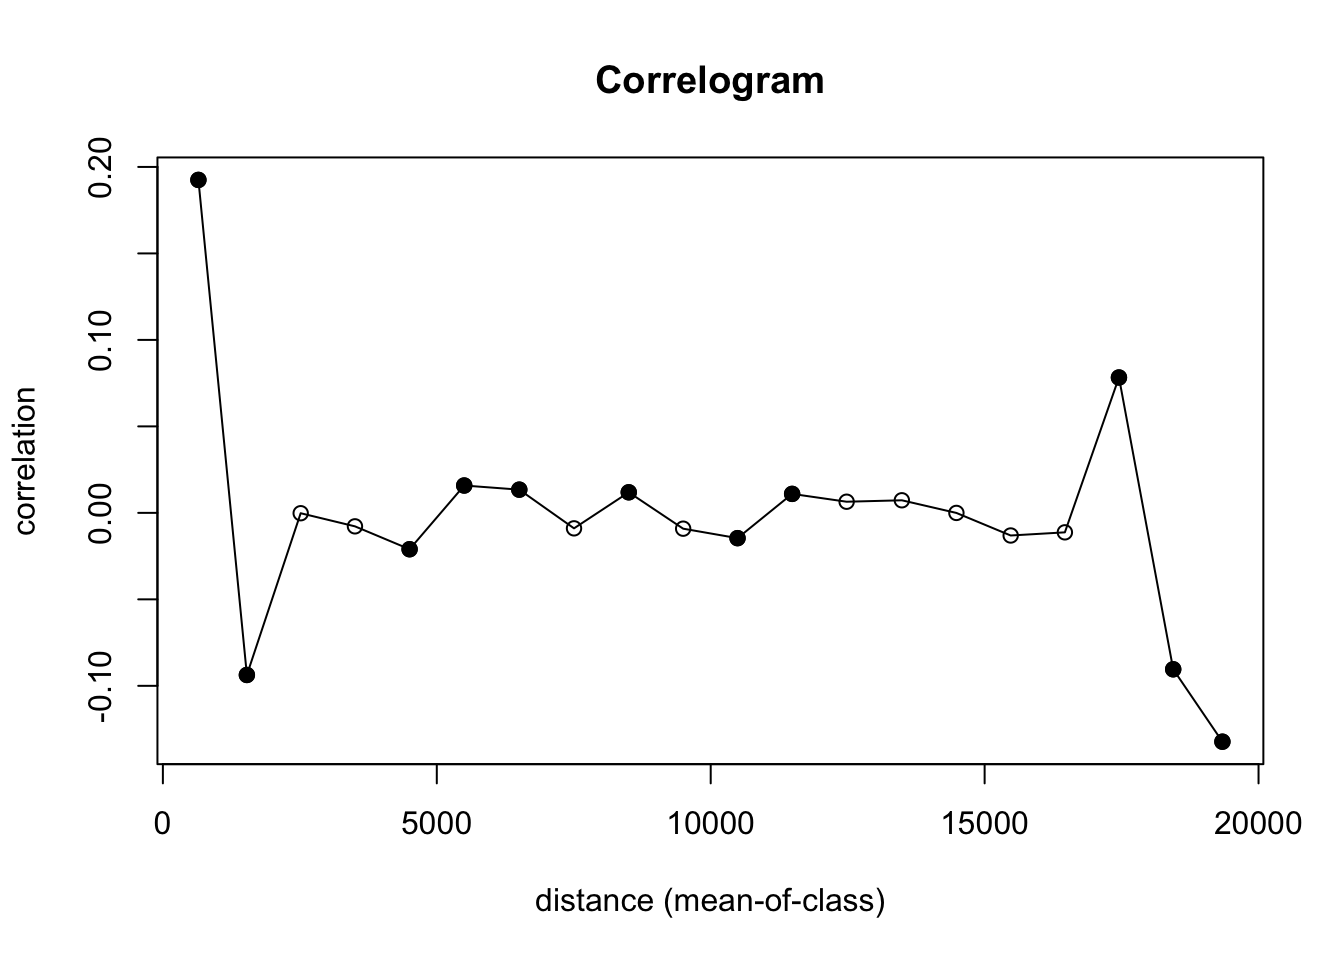
\includegraphics{tutorial_1_files/figure-latex/unnamed-chunk-40-1.pdf}

You can turn the grid of the raster into a spatial object itself, using
the \texttt{as()} function, just as we did for the sf objects before.
Let's do that and plot it on top of the Luxembourg polygon:

\begin{Shaded}
\begin{Highlighting}[]
\NormalTok{z_spatial =}\StringTok{ }\KeywordTok{as}\NormalTok{(z, }\StringTok{'SpatialPolygonsDataFrame'}\NormalTok{)}
\KeywordTok{plot}\NormalTok{(lux_spatial,}\DataTypeTok{axes =}\NormalTok{ T)}
\KeywordTok{plot}\NormalTok{(z_spatial, }\DataTypeTok{add=}\OtherTok{TRUE}\NormalTok{, }\DataTypeTok{border=}\StringTok{'blue'}\NormalTok{, }\DataTypeTok{lwd=}\DecValTok{5}\NormalTok{)}
\end{Highlighting}
\end{Shaded}

\includegraphics{tutorial_1_files/figure-latex/unnamed-chunk-41-1.pdf}

There are several useful functions when working with polygons, e.g.~the
\texttt{aggregate()} function, which can be used to join polygons based
on their values. Let's use that function to join the area polygons by
their values in the \texttt{NAME\_1} column (larger regions):

\begin{Shaded}
\begin{Highlighting}[]
\NormalTok{counties =}\StringTok{ }\KeywordTok{aggregate}\NormalTok{(lux_spatial, }\DataTypeTok{by=}\StringTok{'NAME_1'}\NormalTok{)}
\KeywordTok{plot}\NormalTok{(counties, }\DataTypeTok{col=}\KeywordTok{c}\NormalTok{(}\StringTok{'blue'}\NormalTok{,}\StringTok{'red'}\NormalTok{,}\StringTok{'orange'}\NormalTok{), }\DataTypeTok{lwd=}\DecValTok{3}\NormalTok{, }\DataTypeTok{border=}\StringTok{'black'}\NormalTok{,}\DataTypeTok{axes =}\NormalTok{ T)}
\end{Highlighting}
\end{Shaded}

\includegraphics{tutorial_1_files/figure-latex/unnamed-chunk-42-1.pdf}

We can also determine the overlap of multiple spatial objects. E.g. we
can remove the overlap between two polygons using the \texttt{erase()}
functions. Here we remove the overlap between the map of Luxembourg and
the second cell from our grid that we defined above:

\begin{Shaded}
\begin{Highlighting}[]
\NormalTok{e <-}\StringTok{ }\KeywordTok{erase}\NormalTok{(lux_spatial, z_spatial[}\DecValTok{2}\NormalTok{,])}
\KeywordTok{plot}\NormalTok{(e,}\DataTypeTok{axes =}\NormalTok{ T)}
\end{Highlighting}
\end{Shaded}

\includegraphics{tutorial_1_files/figure-latex/unnamed-chunk-43-1.pdf}

The \texttt{intersect()} function on the other hand does basically the
opposite and keeps only what's shared between two polygons. Using this
function we can e.g.~extract the part of the map of Luxembourg that
falls into our second cell of the made-up grid:

\begin{Shaded}
\begin{Highlighting}[]
\NormalTok{i <-}\StringTok{ }\KeywordTok{intersect}\NormalTok{(lux_spatial, z_spatial[}\DecValTok{2}\NormalTok{,])}
\KeywordTok{plot}\NormalTok{(i,}\DataTypeTok{axes =}\NormalTok{ T)}
\end{Highlighting}
\end{Shaded}

\includegraphics{tutorial_1_files/figure-latex/unnamed-chunk-44-1.pdf}

We can also simply define a rectangle (here we made up some coordinates
that are within the range of the coordinate system of the Luxembourg)
and extract the region covered by that rectangle. We can use the
\texttt{crop()} (or the \texttt{intersect()}) function to extract the
region covered by the rectangle. We define this to a separate variable
(\texttt{pe}) and then plot it in a different color on top of the rest
of the map (in blue). Add the end we also plot the actual rectangle on
top of everything (in red).

\begin{Shaded}
\begin{Highlighting}[]
\NormalTok{e <-}\StringTok{ }\KeywordTok{extent}\NormalTok{(}\DecValTok{6}\NormalTok{, }\FloatTok{6.4}\NormalTok{, }\FloatTok{49.7}\NormalTok{, }\DecValTok{50}\NormalTok{)}
\NormalTok{pe <-}\StringTok{ }\KeywordTok{crop}\NormalTok{(lux_spatial, e)}
\KeywordTok{plot}\NormalTok{(lux_spatial,}\DataTypeTok{axes =}\NormalTok{ T)}
\KeywordTok{plot}\NormalTok{(pe, }\DataTypeTok{col=}\StringTok{'light blue'}\NormalTok{, }\DataTypeTok{add=}\OtherTok{TRUE}\NormalTok{)}
\KeywordTok{plot}\NormalTok{(e, }\DataTypeTok{add=}\OtherTok{TRUE}\NormalTok{, }\DataTypeTok{lwd=}\DecValTok{3}\NormalTok{, }\DataTypeTok{col=}\StringTok{'red'}\NormalTok{)}
\end{Highlighting}
\end{Shaded}

\includegraphics{tutorial_1_files/figure-latex/unnamed-chunk-45-1.pdf}

Another polygon-overlap function is the \texttt{union()} function, which
can be used to merge the spatial information stored in two spatial
objects. As you can see in the plot below, this function creates new
polygon objects from the two input objects which are defined by the
borders of both of these objects. E.g. a region that was defined within
out \texttt{lux\_spatial} object is split into two, if an edge of the
vectorized grid-object \texttt{z\_spatial} runs through it.

\begin{Shaded}
\begin{Highlighting}[]
\NormalTok{u <-}\StringTok{ }\KeywordTok{union}\NormalTok{(lux_spatial, z_spatial)}
\NormalTok{u}
\end{Highlighting}
\end{Shaded}

\begin{verbatim}
## class       : SpatialPolygonsDataFrame 
## features    : 28 
## extent      : 5.74414, 6.528252, 49.44781, 50.18162  (xmin, xmax, ymin, ymax)
## coord. ref. : +proj=longlat +datum=WGS84 +no_defs +ellps=WGS84 +towgs84=0,0,0 
## variables   : 6
## names       : layer, ID_1,     NAME_1, ID_2,   NAME_2, AREA 
## min values  :     1,    1,   Diekirch,    1, Capellen,   76 
## max values  :     4,    3, Luxembourg,   12,    Wiltz,  312
\end{verbatim}

You can see that this created 28 different polygons (compared to the 12
we had before). To make them better visible let's plot them in different
colors.

\textbf{Assigning random colors:} When you have a bunch of different
polygons stored in a \texttt{SpatialPolygonsDataFrame} object and you
want to plot them all in different colors, it can be quite painstaking
to manually define colors for each and single one of them. An easy way
around that is to use a random color generator. E.g. you can sample 100
random colors from the whole color spectrum using the
\texttt{sample(rainbow(100))} command. If you want to use this to assign
colors to polygons in a \texttt{SpatialPolygonsDataFrame} the lost of
colors needs to have the same length as the number of polygons in your
dataframe. To achieve this you can use the \texttt{length()} function to
get the exact number of polygons in your spatial object:
\texttt{sample(rainbow(length(name\_of\_spatial\_object)))}

\begin{Shaded}
\begin{Highlighting}[]
\KeywordTok{plot}\NormalTok{(u,}\DataTypeTok{col=}\KeywordTok{sample}\NormalTok{(}\KeywordTok{rainbow}\NormalTok{(}\KeywordTok{length}\NormalTok{(u))),}\DataTypeTok{axes =}\NormalTok{ T)}
\end{Highlighting}
\end{Shaded}

\includegraphics{tutorial_1_files/figure-latex/unnamed-chunk-47-1.pdf}

The \texttt{cover()} function is a combination between the
\texttt{intersect()} and \texttt{union()} functions. It takes the outer
boundary of the polygon of the first object and intersects it with the
second object, defining new polygons based on the intersect.

\begin{Shaded}
\begin{Highlighting}[]
\NormalTok{cov <-}\StringTok{ }\KeywordTok{cover}\NormalTok{(lux_spatial, z_spatial)}
\NormalTok{cov}
\end{Highlighting}
\end{Shaded}

\begin{verbatim}
## class       : SpatialPolygonsDataFrame 
## features    : 6 
## extent      : 5.74414, 6.528252, 49.44781, 50.18162  (xmin, xmax, ymin, ymax)
## coord. ref. : +proj=longlat +datum=WGS84 +no_defs +ellps=WGS84 +towgs84=0,0,0 
## variables   : 6
## names       : ID_1,       NAME_1, ID_2,     NAME_2, AREA, layer 
## min values  :    1,     Diekirch,    1,   Clervaux,  188,     1 
## max values  :    2, Grevenmacher,    6, Echternach,  312,     4
\end{verbatim}

\begin{Shaded}
\begin{Highlighting}[]
\KeywordTok{plot}\NormalTok{(cov,}\DataTypeTok{axes =}\NormalTok{ T)}
\end{Highlighting}
\end{Shaded}

\includegraphics{tutorial_1_files/figure-latex/unnamed-chunk-48-1.pdf}

\hypertarget{spatial-queries}{%
\subsubsection{Spatial queries}\label{spatial-queries}}

Let's define a set of 5 points and then check which of the polygons they
fall into. First we define the points and convert them into a
\texttt{SpatialPoints} object:

\begin{Shaded}
\begin{Highlighting}[]
\NormalTok{lon =}\StringTok{ }\KeywordTok{c}\NormalTok{(}\DecValTok{6}\NormalTok{, }\FloatTok{6.1}\NormalTok{, }\FloatTok{5.9}\NormalTok{, }\FloatTok{5.7}\NormalTok{, }\FloatTok{6.4}\NormalTok{)}
\NormalTok{lat =}\StringTok{ }\KeywordTok{c}\NormalTok{(}\DecValTok{50}\NormalTok{, }\FloatTok{49.9}\NormalTok{, }\FloatTok{49.8}\NormalTok{, }\FloatTok{49.7}\NormalTok{, }\FloatTok{49.5}\NormalTok{)}
\NormalTok{pts <-}\StringTok{ }\KeywordTok{cbind}\NormalTok{(lon,lat)}
\NormalTok{pts}
\end{Highlighting}
\end{Shaded}

\begin{verbatim}
##      lon  lat
## [1,] 6.0 50.0
## [2,] 6.1 49.9
## [3,] 5.9 49.8
## [4,] 5.7 49.7
## [5,] 6.4 49.5
\end{verbatim}

\begin{Shaded}
\begin{Highlighting}[]
\NormalTok{spts <-}\StringTok{ }\KeywordTok{SpatialPoints}\NormalTok{(pts)}
\KeywordTok{plot}\NormalTok{(lux_spatial, }\DataTypeTok{col=}\StringTok{'blue'}\NormalTok{, }\DataTypeTok{lwd=}\DecValTok{2}\NormalTok{,}\DataTypeTok{axes=}\NormalTok{T)}
\KeywordTok{points}\NormalTok{(spts, }\DataTypeTok{col=}\StringTok{'light gray'}\NormalTok{, }\DataTypeTok{pch=}\DecValTok{20}\NormalTok{)}
\KeywordTok{text}\NormalTok{(spts, }\KeywordTok{c}\NormalTok{(}\DecValTok{1}\NormalTok{,}\DecValTok{2}\NormalTok{,}\DecValTok{3}\NormalTok{,}\DecValTok{4}\NormalTok{,}\DecValTok{5}\NormalTok{), }\DataTypeTok{col=}\StringTok{'red'}\NormalTok{, }\DataTypeTok{cex=}\FloatTok{1.5}\NormalTok{,}\DataTypeTok{pos=}\DecValTok{4}\NormalTok{)}
\end{Highlighting}
\end{Shaded}

\includegraphics{tutorial_1_files/figure-latex/unnamed-chunk-49-1.pdf}

Now we can use the \texttt{over()} function in order to check if and
where each point in our \texttt{SpatialPoints} object intersects with
the \texttt{lux\_spatial} polygon. The function will return a dataframe
that shows for each point the values of the intersecting polygon
dataframe. It will return the value \texttt{NA} for all data columns if
the point did not match any of the polygon

The \texttt{over()} function will complain if the two objects don't have
the same assigned coordinate reference system (CRS). We therefore first
need to assign the correct coordinate reference system to the
\texttt{SpatialPoints} object by using the \texttt{proj4string=} setting
in the \texttt{SpatialPoints()} command. We will assign the same
reference system as the Luxembourg shape object, which we can call by
using the \texttt{crs()} function.

\begin{Shaded}
\begin{Highlighting}[]
\NormalTok{spts <-}\StringTok{ }\KeywordTok{SpatialPoints}\NormalTok{(pts, }\DataTypeTok{proj4string=}\KeywordTok{crs}\NormalTok{(lux_spatial))}
\NormalTok{my_over_output =}\StringTok{ }\KeywordTok{over}\NormalTok{(spts, lux_spatial)}
\NormalTok{my_over_output}
\end{Highlighting}
\end{Shaded}

\begin{verbatim}
##   ID_1   NAME_1 ID_2   NAME_2 AREA
## 1    1 Diekirch    5    Wiltz  263
## 2    1 Diekirch    2 Diekirch  218
## 3    1 Diekirch    3  Redange  259
## 4   NA     <NA>   NA     <NA>   NA
## 5   NA     <NA>   NA     <NA>   NA
\end{verbatim}

\textbf{Task:} Plot only the regions that contain a point, based on the
\texttt{over()} output. The final plot should look like the one below:

Tip: Depending on how familiar you are with R or other programming
languages, you may be able to do this without the instructions below.
Maybe first give it a shot and if you get stuck, have a look at the
instructions below.

One approach would be:

\begin{enumerate}
\def\labelenumi{\arabic{enumi}.}
\item
  Extract the list of region names of the matching polygons from the
  \texttt{over()} function output (make sure you extract a data column
  that enables you to uniquely identify each region). You extract a
  specific data column using the \texttt{\$column\_name} notation
  following the name of the object, e.g.
  \texttt{my\_over\_output\$ID\_1} extracts the column \texttt{ID\_1}
  from the \texttt{my\_over\_output} object.
\item
  Identify which of the polygons in the \texttt{lux\_spatial} object
  match this list of target regions. You can use the \texttt{which()}
  function to determine the polygon indeces that fulfil a given
  requirement. In order to define a requirement you can use the
  \texttt{\%in\%} notation to test which elements from one list match
  with elements from another, e.g.
  \texttt{which(lux\_spatial\$NAME\_2\ \%in\%\ my\_list\_of\_target\_regions)}
  returns the indeces of those polygons, whose name is present in the
  list \texttt{my\_list\_of\_target\_regions}.
\item
  Extract the target polygons from the \texttt{lux\_spatial} object. Use
  the indeces that where produced by the \texttt{which()} command to
  index the polygons you want to extract, e.g.
  \texttt{lux\_spatial{[}list\_indeces,{]}} extracts all indeces present
  in the list \texttt{list\_indeces}.
\end{enumerate}

\includegraphics{tutorial_1_files/figure-latex/unnamed-chunk-51-1.pdf}

\hypertarget{working-with-raster-data}{%
\subsubsection{6. Working with raster
data}\label{working-with-raster-data}}

It's rather straight-forward to generate a raster in R. As we did
earlier in this tutorial we can just create a raster by using the
\texttt{raster()} command and specifying the number of cells and extent
in x and y direction. Remember that this command only creates the
skeleton (empty raster). Here we just fill these cells with random
numbers between 0 and 1 using the \texttt{runif()} command.

\begin{Shaded}
\begin{Highlighting}[]
\NormalTok{x <-}\StringTok{ }\KeywordTok{raster}\NormalTok{(}\DataTypeTok{ncol=}\DecValTok{36}\NormalTok{, }\DataTypeTok{nrow=}\DecValTok{18}\NormalTok{, }\DataTypeTok{xmn=}\OperatorTok{-}\DecValTok{1000}\NormalTok{, }\DataTypeTok{xmx=}\DecValTok{1000}\NormalTok{, }\DataTypeTok{ymn=}\OperatorTok{-}\DecValTok{100}\NormalTok{, }\DataTypeTok{ymx=}\DecValTok{900}\NormalTok{)}
\KeywordTok{values}\NormalTok{(x) <-}\StringTok{ }\KeywordTok{runif}\NormalTok{(}\KeywordTok{ncell}\NormalTok{(x))}
\KeywordTok{plot}\NormalTok{(x)}
\end{Highlighting}
\end{Shaded}

\includegraphics{tutorial_1_files/figure-latex/unnamed-chunk-52-1.pdf}

You can check the resolution of the raster (dimensions of each cell)
using the \texttt{res()} command:

\begin{Shaded}
\begin{Highlighting}[]
\KeywordTok{res}\NormalTok{(x)}
\end{Highlighting}
\end{Shaded}

\begin{verbatim}
## [1] 55.55556 55.55556
\end{verbatim}

It turns out each of our cells has the size 55.5x55.5, i.e.~it covers
55.5 units on the x-axis and 55.5 untis on the y-axis. You can change
the resolution of the raster. Let's change it to \texttt{1}, which will
lead to many more cells in the raster, as the cells will now only have
the size 1x1 and fill the cells with random values.

\begin{Shaded}
\begin{Highlighting}[]
\KeywordTok{res}\NormalTok{(x) <-}\StringTok{ }\DecValTok{1}
\KeywordTok{values}\NormalTok{(x) <-}\StringTok{ }\KeywordTok{runif}\NormalTok{(}\KeywordTok{ncell}\NormalTok{(x))}
\KeywordTok{plot}\NormalTok{(x)}
\end{Highlighting}
\end{Shaded}

\includegraphics{tutorial_1_files/figure-latex/unnamed-chunk-54-1.pdf}

We can access the coordinate projection of the raster using the
\texttt{projection()} function and can assign a value to it (see
\href{http://rspatial.org/spatial/rst/6-crs.html}{this link from
earlier} to check again the notation for different coordinate reference
systems). There will be a more thorough explanation of how to decide
which projection to assign to your spatial object in the next tutorial.

\begin{Shaded}
\begin{Highlighting}[]
\KeywordTok{projection}\NormalTok{(x) <-}\StringTok{ "+proj=utm +zone=48 +datum=WGS84"}
\KeywordTok{projection}\NormalTok{(x)}
\end{Highlighting}
\end{Shaded}

\begin{verbatim}
## [1] "+proj=utm +zone=48 +datum=WGS84 +ellps=WGS84 +towgs84=0,0,0"
\end{verbatim}

Summary of some useful basic raster commands:

\begin{itemize}
\tightlist
\item
  \textbf{res()} - access the raster resolution (cell dimensions)
\item
  \textbf{projection()} - access the coordinate projection of the raster
\item
  \textbf{ncell()} - access the number of cells in the raster
\item
  \textbf{ncol()} - access the number of columns in the raster
\item
  \textbf{dim()} - access the dimension of the raster (cells in x and y
  direction)
\item
  \textbf{values()} - access the values stored in the raster cells
\item
  \textbf{hasValues()} - check if raster contains values or if it's just
  an empty skeleton
\item
  \textbf{xmax()} - access the maximum x value
\item
  \textbf{xmin()} - \ldots{}
\item
  \textbf{ymax()} - \ldots{}
\item
  \textbf{ymin()} - \ldots{}
\end{itemize}

We can stack multiple rasters into the same object by using the
\texttt{stack()} command. Here we define 3 rasters with random numbers
and stack them:

\begin{Shaded}
\begin{Highlighting}[]
\NormalTok{r1 <-}\StringTok{ }\NormalTok{r2 <-}\StringTok{ }\NormalTok{r3 <-}\StringTok{ }\KeywordTok{raster}\NormalTok{(}\DataTypeTok{nrow=}\DecValTok{10}\NormalTok{, }\DataTypeTok{ncol=}\DecValTok{10}\NormalTok{)}

\CommentTok{# Assign random cell values}
\KeywordTok{values}\NormalTok{(r1) <-}\StringTok{ }\KeywordTok{runif}\NormalTok{(}\KeywordTok{ncell}\NormalTok{(r1))}
\KeywordTok{values}\NormalTok{(r2) <-}\StringTok{ }\KeywordTok{runif}\NormalTok{(}\KeywordTok{ncell}\NormalTok{(r2))}
\KeywordTok{values}\NormalTok{(r3) <-}\StringTok{ }\KeywordTok{runif}\NormalTok{(}\KeywordTok{ncell}\NormalTok{(r3))}

\NormalTok{s <-}\StringTok{ }\KeywordTok{stack}\NormalTok{(r1, r2, r3)}
\KeywordTok{plot}\NormalTok{(s)}
\end{Highlighting}
\end{Shaded}

\includegraphics{tutorial_1_files/figure-latex/unnamed-chunk-56-1.pdf}

\hypertarget{algebraic-operations-with-rasters}{%
\paragraph{Algebraic operations with
rasters}\label{algebraic-operations-with-rasters}}

Rasters are very straightforward to work with, since they allow the use
of simple algebraic operators such as +, -, *, /, as well as logical
operators such as \textgreater{}, \textgreater{}=, \textless{}, ==, !.

For example if we want to add the values across all 3 rasters from above
we can simply do that like this:

\begin{Shaded}
\begin{Highlighting}[]
\NormalTok{sum_rasters =}\StringTok{ }\NormalTok{r1 }\OperatorTok{+}\StringTok{ }\NormalTok{r2 }\OperatorTok{+}\StringTok{ }\NormalTok{r3}
\CommentTok{# or:}
\NormalTok{sum_rasters =}\StringTok{ }\KeywordTok{sum}\NormalTok{(r1, r2, r3)}
\KeywordTok{plot}\NormalTok{(sum_rasters)}
\end{Highlighting}
\end{Shaded}

\includegraphics{tutorial_1_files/figure-latex/unnamed-chunk-57-1.pdf}

Congratulations, you made it through the first tutorial! Here you can
move on to the \href{./tutorial_2.html}{next tutorial}, using real data.


\end{document}
